%
% include the class file for GMP 2015
%
\documentclass[final]{gmp2015}

%%%%%%%%%%%%%%%%%%%%%%%%%%%%%%%%%%%%%%%%%%%%%%%%%%%%%%%%%%%%%%%%%%%%

%\usepackage{t1enc,dfadobe}

%\usepackage{egweblnk}
\usepackage{cite}

\usepackage{graphicx}



\graphicspath{{./Figures/}}

%\usepackage[scaled=.92]{helvet}B
%\usepackage{times}
%\usepackage{bm}
\usepackage{algorithm}
\usepackage{algorithmic}
%\usepackage{multirow}
%\usepackage{amsmath,amssymb,amsfonts,euscript,mathrsfs}
%\usepackage{hhline}

\usepackage{./picins/picins}
%\usepackage{picinpar}
\usepackage{subfigure}
\usepackage[symbol*]{footmisc}
%\let\theoremstyle\relax
%\usepackage{ntheorem}
%\usepackage{bbding}
%\usepackage{mathptmx}
%\usepackage{soul}

%\usepackage{color}
%\definecolor{turquoise}{cmyk}{0.65,0,0.1,0.1}
%\definecolor{purple}{rgb}{0.65,0,0.65}
%\definecolor{dark_green}{rgb}{0, 0.5, 0}
%\definecolor{orange}{rgb}{0.8, 0.2, 0.2}

%\newcommand{\ligang}[1]{{\color{orange}[Ligang:  #1]}}
%\newcommand{\zhouwang}[1]{{\color{blue}[Zhouwang: #1]}}
%\newcommand{\xuefeng}[1]{{\color{red}[Xuefeng: #1]}}
%\newcommand{\liuyuan}[1]{{\color{purple}[Liuyuan: #1]}}
%\newcommand{\tuanfeng}[1]{{\color{purple}[Tuanfeng: #1]}}
%\newcommand{\tofix}[1]{{\color{red}[#1]}}
%
%\newcommand{\ca}[1]{{\color{red}            {#1}}}
%\newcommand{\cb}[1]{{\color{blue}            {#1}}}


%\long\def\nix#1{\relax}


\title{Global Stiffness Structural Optimization for 3D Printing under Unknown Loads}





%
% put the title of your paper here
%
%\title{A nice paper that is being submitted to GMP 2015}

%
% put your submission number here
% this number will appear instead of authors and affiliations if the class option "submission" is active
%
\SubNumber{69}

%
% put the author names here
% use the second argument as a reference to the list of affiliations
% no authors and affiliations will appear if the class option "submission" is active
%
\author{Tuanfeng Y.\ Wang}{1,2}
\footnotetext{Email:Tuanfeng.wang@cs.ucl.ac.uk}
\author{Yuan Liu}{1}
\author{Xuefeng Liu}{3}
\author{Dongming Yan}{4}
\author{Ligang Liu}{1}
\author{Jiansong Deng}{1}
\author{Falai Chen}{1}
\author{Zhouwang Yang}{1}


%
% put the affiliations of the authors here
%
\affiliation{1}{University of Science and Technology of China}
\affiliation{2}{University College London}
\affiliation{3}{Niigata University}
\affiliation{4}{VCC, KAUST}

\begin{document}



%
% the rest is as usual
%
\maketitle
%%%%%%%%%%%%%%%%%%%%%%%%%%%%%%%%%%%%%%%%%%%%%%%%%%%%%%%%%%%%%%%%%%%%



\begin{abstract}

%% Abstract

%In this paper, we address the problem of designing a global stiffness structure for an object with a certain amount of the given material for 3D printing.
%%
%We propose a novel solution for the structural optimization problem that computes an optimal structure for all kinds of force distribution.
%Specifically, we use the eigen-mode analysis that maximizes the minimal positive eigenvalue of the stiffness matrix by varying the design variables of the frame structure.
%%
%Furthermore, we present a Rayleigh-quotient based algorithm for accelerating the structural optimization.
%%
%Our approach provides a solution for formulating the adaptive hollowing and the interior supportive structure in a unifed form and optimizing them simultaneously.
%%
%The validity, the rationality and the applicability of our solution are verified by the finite element method analysis and by the mechanical test of printed objects.
%%
%Our approach obtains the global stiffness structures and is shown to be more practical than the state-of-the-art approaches.

%%%%%%%%%%%%%%%%%%%%
The importance of the stiffness of a 3D printed object has been realized gradually nowadays. Unlike industry product using \textit{stiff-but-weak} materials such as metal, cement, etc. using stress as criterion is not suitable when considering the problem of 3D printing as materials used here (ABS, Nylon, resin, etc.) is rather elastic \textendash \  which is the case of \textit{flexible-but-strong}. 3D printed objects are always hollowed with interior structure to make the fabrication process cost-effective while maintain the stiffness. State-of-the-art techniques are either \textit{redundant design} (using an amount of materials much more than necessary to ensure the stiffness in any case) or optimizing the structure under one of the most-possible loads distributions which fall short in other distribution cases. We propose a novel approach for designing the interior of the object by optimizing the global stiffness \textendash \  minimizing the maximum deformation under any possible load distribution. We first simulate the object by a lightweight frame structure and optimize both the size and the geometry using an eigen-mode-like formulation, interleaving with a topology clean. A postprocess is applied to generate the final object based on the optimized frame structure. Optimizing the interior structure under unknown loads automatically keeps reinforce where the structure is the weakest and is proved to be a powerful and more reasonable design framework in our experimental results.

%In this paper, we address the problem of designing a frame structure with optimized stiffness distribution for the 3D printing objects.
%We propose a novel solution to the structural optimization problem that provides minimal deformation of the frame structure under various distributions of force.
%
%Such a solution is obtained in two steps.
%First, we perform an eigen-mode analysis to find the greatest deformation for all normalized distribution of force, which is related to the calculation of the minimal positive eigenvalue of the stiffness matrix.
%First, we perform an eigen-mode analysis to find the region at which the object undergoes the greatest deformation under a normalized distribution of force.
%This result enables us to calculate the minimal positive eigen-value of the stiffness matrix.
%Second, we vary the the design variables of the frame structure to minimize the deformation.
%In this step, a Rayleigh-quotient based algorithm is proposed to accelerate the structural optimization.
%
%The validity and the rationality of our solution are verified by the finite element method analysis and by the mechanical simulation of printed objects.
%Our approach can obtain the global stiffness in structures and is shown to be more applicable than state-of-the-art methods.



%In this paper, we address the problem of designing a frame structure with optimized stiffness distribution for the 3D printing objects. We propose a novel solution to the structural optimization problem that provides minimal deformation of the frame structure under various distributions of force. Such a solution is obtained in two steps. First, we perform an eigen-mode analysis to find the region at which the object undergoes the greatest deformation under a normalized distribution of force. This result enables us to calculate the minimal positive eigen-value of the stiffness matrix. Second, we vary the the design variables of the frame structure to minimize the deformation. In this step, a Rayleigh-quotient based algorithm is proposed to accelerate the structural optimization.
%The validity and the rationality of our solution are verified by the finite element method analysis and by the mechanical simulation of printed objects.
%Our approach can obtain the global stiffness in structures and is shown to be more applicable than state-of-the-art methods.

\end{abstract}

%%%%%%%%%%%%%%%%%%%%%%%%%%%%%%%%%%%%%%%%%%%%%%%%%%%%%%%%%%%%%%%%%%%%


\section{Introduction}
\label{sec:intro}


%% 1. ��ά��ӡ�������ı仯�ǣ����ӵ������ڲ��ṹ��Ʋ������У���ʱҲ�DZ�Ҫ�ġ�

%��ͳ���췽���Ƚ�ƫ���ڱ���ӹ��������и����ڲ��ṹ���������һ�ο��ٳ��͡�
%����Щ����£�Ϊ������������������ܵ��ڲ��ṹ�Ƿdz���Ҫ�ġ�
%������ά��ӡ�����ij��֣����ڸı�������̬�ơ�

The 3D printing technique provides a powerful solution to prototype customized objects with fine surface details and complex interior structures. However, the spread and development of this technique is hindered to the high cost of material and low speed of fabrication. Research efforts have been devoted to reduce the material used, i.e., the volume/weight of object, and the key challenge here is to keep the stiffness while less material is used. Given a load distribution, it is natural to hollow the object for a cost-effective purpose and add interior structure to optimize the structure stiffness-to-weight ratio \cite{stava:2012,wang:2013,Lu:2014}. Such load-distribution-based techniques have been highly successful in ideal cases as prefectly minimizing the structural deformation/stress with much less material in real world plysical test with corresponding preset loads. However, they are not suitable for many real world applications because the loads on a fabricated object may appear in other distributions which are different from the preset one. As shown in Figure~\ref{fig:teaser:a}, the Trophy model could be hold in many different ways which lead to very different load distribution cases. 
 
Instead of taking one (or several) load distribution case(s) into consideration, we optimize the global stiffness-to-weight ratio by minimizing the maximum of deformation under any load distribution cases, named as unknown loads due to no load distribution case is given to be based on. We use the criterion \textit{deformation} rather than \textit{stress}, as the former is more suitable when using elastic materials like many materials in 3D printing. Such elastic property preserve the fabricated object from breaking under large stress but is much easier to be deformed when load is applied. The rationality of the deformation based formulation can coincidently be supported by pervious research as well (see details in Sec.~\ref{subsec:eigen-mode-opt}). When the amount of material is given, our unknown-load-based optimization framework aims to make the object perform the best (stiffest) among other interior design when the corresponding worst (lead to the largest deformation) load disctribution case is appied.

Our work is inspired by the research of \cite{Chen:2007} and \cite{wang:2013}. These work show that an entire object can be simulated by a frame structure consisting of a set of beams and a set of nodes connected by these beams. Frame structure captures most of the structural features of the object and has a rather small set of parameters which can be analyzed and computed with high efficiency. The last step of our framework restores the optimized frame structure back to an entity object ready to be fabricated and the global stiffness property is proved to be kept.

Prior to global stiffness optimization, we first perform a \textit{Constrained Centroidal Voronoi Tessellation} (CCVT) on the input object and obtain an isotropic initial frame by taking the edges of each tetrahedron as beam of the initial frame. The global stiffness problem is then formulated as a saddle point problem by minimizing the maximum norm of the deformation under any normalized load. Optimization on nodes positions, beam radii and nodes topology connections are applied to the frame structure using a saddle point algorithm. After optimization algorithm is terminated, we adopt a postprocess step to generate the object with original object surface and lightweight interior based on the optmized frame structure. Note that it is not simply cover a skin on the frame structure like \cite{wang:2013}. As the skin can not be analyzed efficiently, our postprocess is rather like an adaptive hollowing meanwhile adding interior supportive structure. Finally, we use the \emph{Finite Element Method} (FEM) to analyze and verify the rationality of our results.





%Such objects are difficult to fabricate using traditional manufacturing systems, which lay particular emphasis on surface processing.
%The objects with complex interior structures are difficult to be fabricated by traditional manufacture methods
%which pay more emphasis on shaping and surface processing.
%In some cases, it is required to hollow the objeect and design the interior structure for a cost-effective purpose \cite{wang:2013} or to meet specific functional goals \cite{bacher2014spin}.
%The capability of using digital representations to generate solid objects with fine surface details and complex interior structures inspires significant effort.
%
%Technologies around 3D printing have received a lot of attention unprecedentedly and been popular since recent years.
%In practice, the 3D printing provides a powerful solution to prototype the customized objects with complex interior structure design, which opened new horizons in 3D shape design technologies for fabrication.


%The techniques of Fast Fabrication, also known as 3D printing, have been more and more developed and matured in recent year \cite{relative papers}. No matter what specified technique is used, the basic idea of 3D printing is stacking cross-section layers of an object one by one result in when comparing with traditional processing methods like CNC, etc., 3D printing is able to build complex interior structure with highly flexible. It makes the problem of interior structure design for achieving some customized properties receive a lot of attention unprecedentedly.

%As the raw material input to 3D printer remain expensive but reusable, the production cost of the resulting model is directly related to the volume of target object without much impact on the printing process (wasted material is reusable). Take this factor into consideration, the designing of cost effective 3D shapes by reducing their interior material (i.e. achieving some customized properties with minimal material cost) has been studied recently like \cite{wang:2013,buildtolast}, which is called cost-effective structure optimization.



%% 2. �����ľ��������ع�����������ָ�������µĽṹ�������Ż�������ʵ����ǣ�������������ܻ��ܵ����ֲ�����Ԥ���������á�



%In fabrication engineering, extensive attention has been paid to shape analysis and structural optimization~\cite{Crapo:1979,Rosenberg:1980,Haftka:1986,zhou:2013}.
%Many kinds of lightweight structures, including frames and honeycombs,
%have been developed to reduce weight and reinforce strength~\cite{Kindinger:2001,song:2013,wang:2013}.
%
%However, the vast majority of previous work focuses on structural design and optimization under specified load environments, such as simulated handling, pressure, or evenly distributed force.
%
%Actually, a fabricated object might be handled or used in various possible ways,  which cannot be simulated by an exact load distribution.
%For instance, it is difficult to predict where a football would be kicked during a game and specified loads cannot emulate all cases.
%
%Due to the inability of existing forms of structural optimization to plan for all possible load distributions, current methods have obvious limitations and fail to satisfy the aforementioned situation.
%
%However, previous work on cost-effective structure optimization are focusing on the situation under some given loads including gravity and share the formulation as the given external loads act on the surface on the object to simulate handling, pressing etc., and the gravity act on everywhere of the solid.
%When operating optimization with certain loads, a solid with interior structure is generated which accounts strength under this situation. This formulation is very limited for many cases because for most of the time, people can not predict a exact load distribution when it is used after the fabrication like a football which cannot be decided where it will be kicked during the game or a mobile phone which cannot be told the exact holding position or a bridge which cannot be predict where the heavy car will go. Even for some easy case with only limited possible load distribution, no existing method can synthesize structures generated under each given load distribution. Or if we add all the possible load distributions up together for a single optimization, there is no guarantee of working for the distributions might contradict, e.g. a place on the surface could be pulled in one situation and pushed in another.





%% 3. ����Ż��ṹ���ʹ֮��Ӧ�Ը��ֿ��ܵ��������������Ǻܾ���ս�Ե����⡣
%%    ����������⽨��ȫ�µ��Ż�ģ�ͣ��ṹ����Ʊ�����ģ�ɿز�����Ч�����ǹؼ��㡣
%%    ����frame�ṹ��motivation���ɶ�������м򻯽��ƿ̻�����ѧģ�ͣ�ʹ֮����Ч���㡣
%


%In this paper, we consider the problem of optimizing the structure design of an object such that it can withstand all possible force environment.

%In this paper, we address the problem of designing a global stiffness structure for an object
%under unprescribed loads when a certain amount of material is given.
%
%The main challenges of this problem include:
%(1) establishing an effective model with design variables of controllable scale to appropriately characterize the problem;
%(2) developing an efficient algorithm to solve the model and attain optimally designed structures;
%and (3) verifying the rationality and validity of the obtained results.



%% 4. �������ĵķ������乱�ס�


%In this paper, we proposed a novel formulation for optimize the structure under a given material bound that the designed structure will be damaged least is a bounded load under any possible most-damaged load distribution which can be also described as optimizing the worst case to the best. The designed solid is considered as an adaptive hollowing surface with cylinder-like interior supportive structure. In order to get this problem solvable, we simulate the structure via frame. The adaptive-hollowed surface is simplified as a mesh-like surface frame with different radius on each beams and the interior structure is connected beams in the surface frame.



%We propose a novel approach that formulates the structural optimization problem by maximizing the total potential energy of a target structure, consisting of an adaptive hollowed surface shell and interior supportive beams.
%
%The designed structure can be well simulated via frame structure~\cite{wang:2013}, which simply approximates the adaptive hollowed surface shell and interior beams as  a unified form.
%In order to get this problem solvable, we simulate the structure via frame.
%The adaptive hollowed surface is simplified as a mesh-like surface frame with different radius on each beams
%and the interior structure is connected beams in the surface frame.
%
%Then the structural optimization is reformulated as a saddle point model, i.e., by maximizing the minimum non-zero eigenvalue of the stiffness matrix from the designed frame structure.
%
%We present an algorithm based on the Rayleigh-quotient to solve the saddle point model efficiently and obtain the final structure with optimal design variables (i.e., the beam radii and the node position).
%
%Finally, we use the \emph{Finite Element Method} (FEM) to analyze and verify the rationality of our results.


%We utilize the dual triangulation of centroidal Voronoi diagram with uniform density function to generate an initial guess of the frame.
%
%The optimization problem adjust the frame parameter (node position and radius of beams) , essentially, to minimize the largest compliance under any load distribution.
%
%We prove that the optimization problem can be equivalent to the optimizing of critical value of Rayleigh quotient which is linear and explicit.
%
%After casting the optimization problem as mutually finding an optimal distribution of the radius of frame's edges and the position of each nodes under a total volume constrain, the result frame will lead the generation of output solid in the end.
%
%Further more, with a simple outer loop, our method is also available for the goal of minimize the material cost under the constraint of minimal load-bearing performance. We will show that the largest compliance can be calculated with the worst load distribution, a binary chop can then be added as a outer loop to find the minimal cost for a upper bound of compliance.





%\begin{itemize}
%\item We first work on the problem of cost-effective structure optimization under unknown load distribution and formulate the optimization problem on getting the best strength under worst situation.
%
%\item The optimization problem is time consuming under a naive solving method, we use the concept of Rayleigh quotient to transfer the implicit eigenvalue problem into explicit Rayleigh-quotient formulation.
%
%\item We proposed the first method on organize the adaptive hollowing and interior structure in an uniform form and optimize them together.
%\end{itemize}


\begin{figure*}[t]
  \centering
  \subfigure[]{
          \label{fig:teaser:a}
          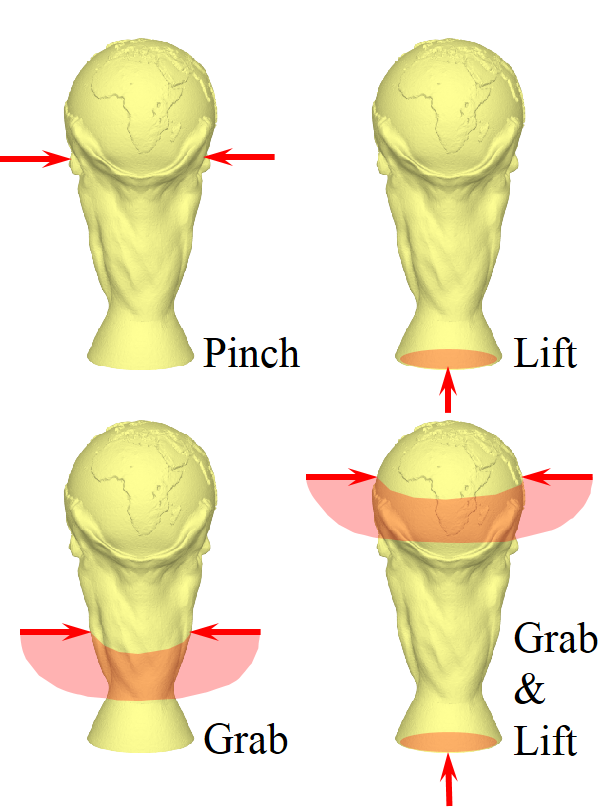
\includegraphics[width=.2236\linewidth]{Figures/teaser/teaser_1.png}
  }\quad
  \subfigure[]{
          \label{fig:teaser:b}
          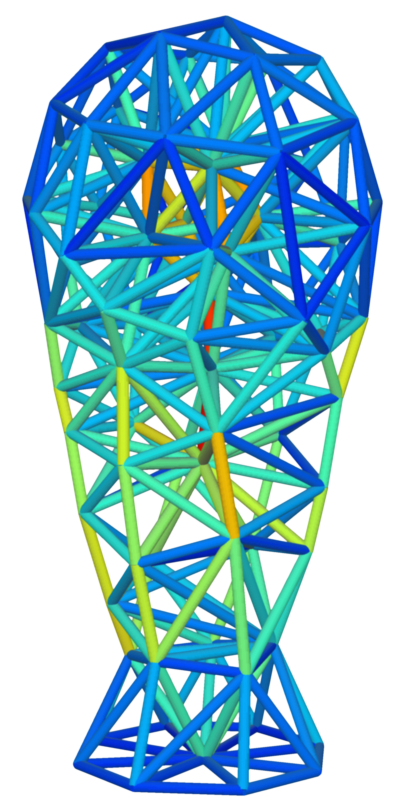
\includegraphics[width=.1465\linewidth]{Figures/teaser/teaser_2.png}
  }\quad
  \subfigure[]{
          \label{fig:teaser:c}
          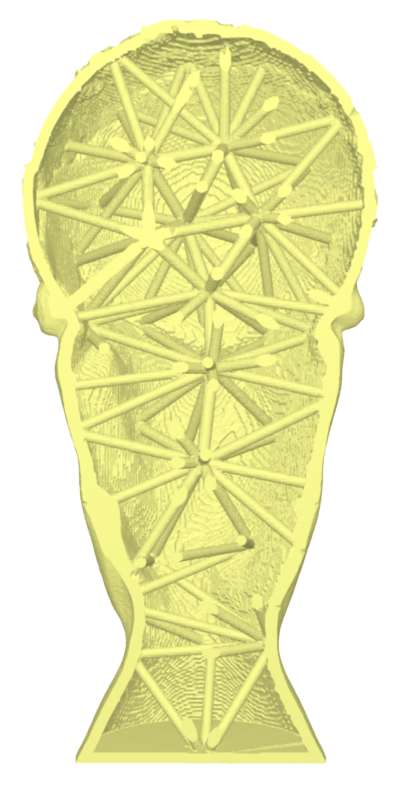
\includegraphics[width=.1465\linewidth]{Figures/teaser/teaser_3.png}
    }\quad
  \subfigure[]{
          \label{fig:teaser:d}
          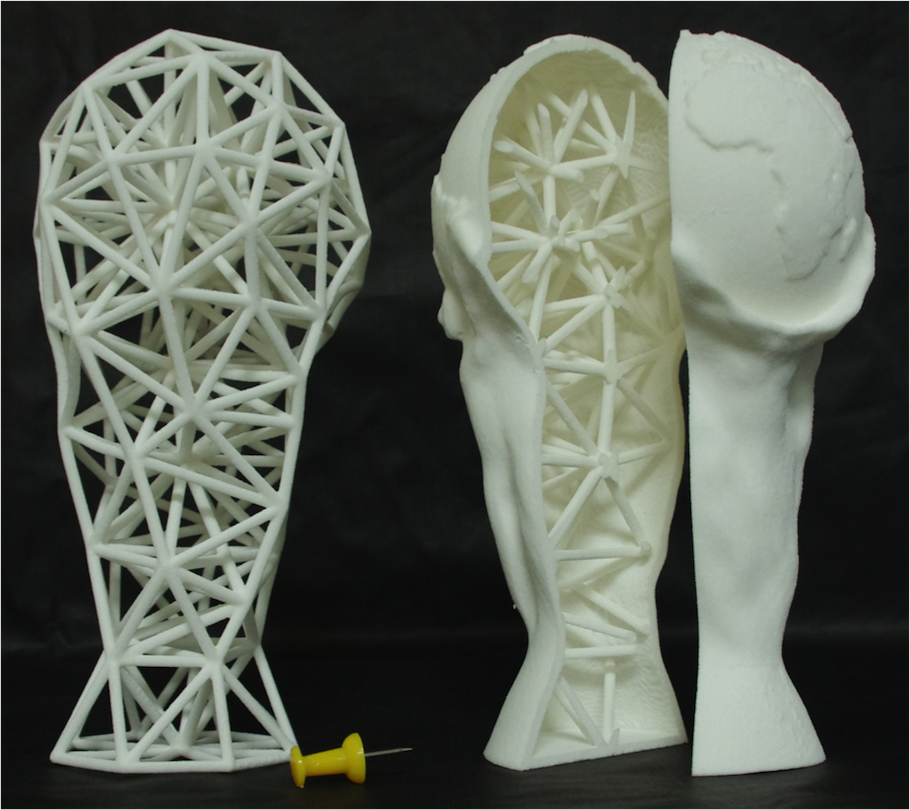
\includegraphics[width=.3334\linewidth]{Figures/teaser/teaser_4.png}
  }\quad

  \caption{\label{fig:teaser}
  For the Trophy model (a), a user could hold it in many possible gestures but this remains uncertain during the interior  design for a cost-effective purpose. With a given amount of material, our algorithm first produces a global stiffness frame structure (b) under unknown loads, by minimizing the maximal deformation (colored accroding to beam radii). (c) is the sectional view of the object generated from the optimized frame structure, and (d) is the photo of the printed frame and the object generated by our method. A yellow standard pin is placed next to the object as the size reference. }
\end{figure*}

\section{Related Work}
\label{sec:related}


%\hl{Technologies around 3D printing have been popular since recent years. The capability of generating tangible solid objects with fine surface details and complex interior structures from their digital representation inspires significant efforts in relative areas. In practice, 3D printers are a powerful and affordable commercial solution to popularize the self-prototyping of custom-designed sphtsical objects and complex inner structure design, which opened new horizons in 3D shape design technologies for fabrication.} \zhouwang{move this part to introduction?}


Significant efforts have been made recently on fabrication-aware 3D shape design which establishes physically-fabricated prototypes and manufactured objects using 3D printing. Previous work focused on the desire of certain physical properties, such as deformation behavior~\cite{Bickel:2010}, fabricatable via comercial 3D printer's limited working volume~\cite{luo2012chopper}, physical realization~\cite{stava:2012}, stability over gravity on certain orientation~\cite{prevost:2013, bacher2014spin}. These work fully developed the benefit of 3D printing over traditional CNC fabrication techniques because both fine surface details and complex interior structure are able to be fabricated.

Over the recent years it has been more and more recognized that 3D printing techniques, including FDM/SLS/SLA, etc., are hindered for both research and commercial purposes by such a high material cost and a rather low fabrication speed. The core problem here is to reduce the designed volume of the object. Inspired by lightweight structure observed from nature, \cite{wang:2013, Lu:2014} adopted lightweight structures to fill the object rather than solid interior. These work optimize the stiffness/strength-to-weight ratio under a given external force while the original object surface is preserved. However, the results of these load-based methods fall short in real world cases as load distribution applied by user is always different from the ideal preset case. With a novel formulation, our proposed unknown-load-based method perfectly solves this problem by optimizing and generating a global stiffness design with a uniform framework. Without a given load distribution, \cite{umetani2013cross} presents a structural analysis technique that slice the object into cross-sections and compute stress based on bending momentum equilibrium. For a similiar purpose, a finite element based structural analysis method is presented in~\cite{zhou:2013}. Based on experimental observation, this work uses an Eigenmode formulation to detect the weakest area of an object. In our paper, this observation is proved mathmatically from our global stiffness formulation. In computational structure area, structure analysis and optimization under unknown load distribution have been discussed during the past few years, such as \cite{cherkaev2004principal,cherkaev1998stable,takezawa2011topology}. These work, although sharing the same target, test different kinds of object functions without a proof of rationality. These work also limited the problem into 2D domain and focus on only geometry rather than take all variables (size, geometry, topology) into consideration, which is far from a complete solution of the cost-effective fabrication challenge.

In order to reduce the volume of the object, lightweight structure is adapted for supportive interior. The design and optimization of lightweight structures have been extensively explored in tissue engineering and computer-aided design. 
Smith et al.~\cite{Smith:2002} focus on optimizing the design of truss structures where beams connected by pin joints are rotation-free and difficult to preserve the geometrical shape of the object.
Using lightweight structures for improving the strength and the stiffness of objects has also been studied in the field of rapid manufacturing~\cite{wang:2005}, where the particle swarm optimization or generic algorithm were selected to search for design solutions. Detailed reviews on various aspects of structural optimization can be found in~\cite{bendsoe:2003}. Due to the differences in the types of objectives and constraints, the approaches there in are not suitable for our purpose of 3D printing.

We use the frame structure in the lightweight design for its fabrication-friendly. Each beam in the frame structure is considered as the basic element which is different from classical structural topology optimization methods. Structural topology optimization is employed mainly to specify the optimum number and location of holes in the configuration of the designed structure.
Element-based methods for structural topology optimization decompose the volume of the input object into finite-element-like tetrahedrons, or a grid-like structure for analysis. The \emph{Optimality Criteria} (OC)~\cite{rozvany:1989} methods are proved to be among the most effective element-based methods for solving topology optimization problems. 
A recent review of this area is offered by~\cite{rozvany:2009}.
It is easy to extend our framework into element-based computation, however, due to the linear elastic property of frame structure, taking a single beam as basic element is much more efficient.


\section{Problem and formulation}
\label{sec:formulation}



\begin{figure*}[t]

  \centering
    \subfigure[]{
            \label{fig:pipeline:a}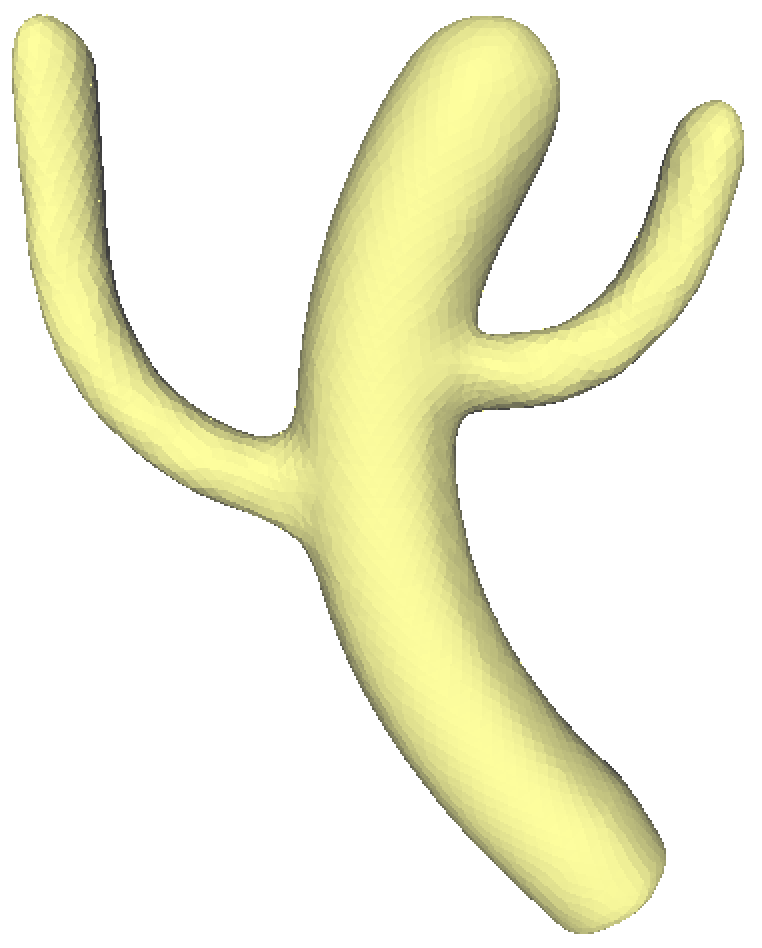
\includegraphics[width=.19\linewidth]{Figures/pipeline/1.png}}\quad
    \label{fig:pipeline:b}\subfigure[]{
            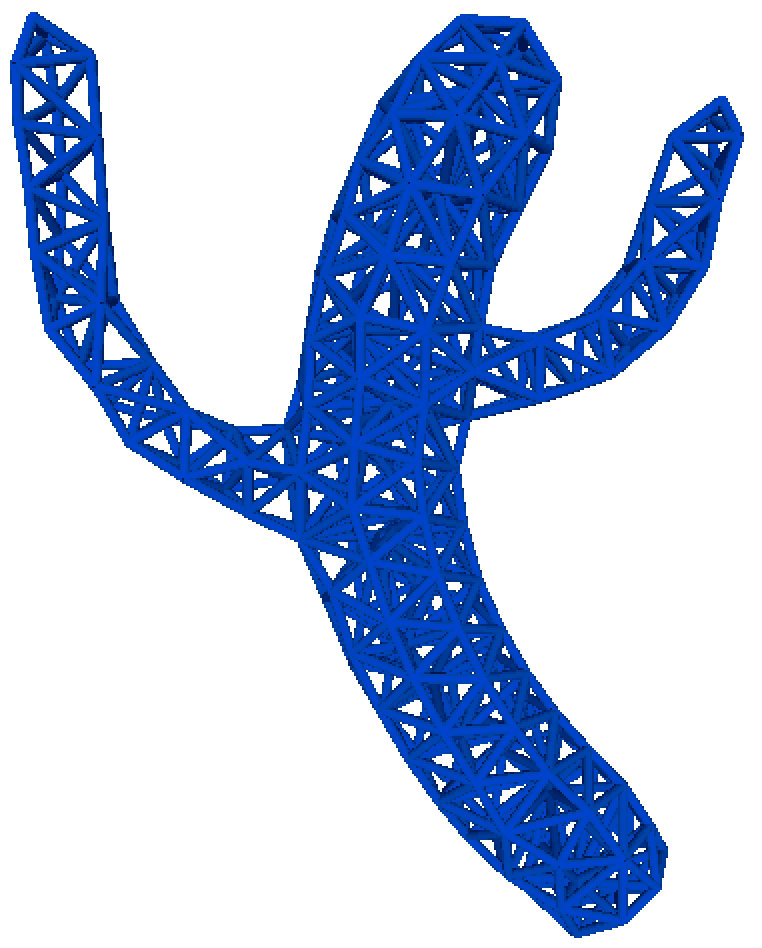
\includegraphics[width=.19\linewidth]{Figures/pipeline/2.png}
            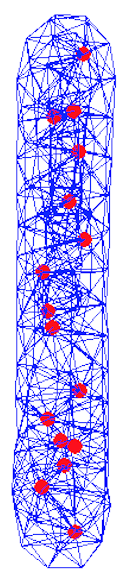
\includegraphics[width=.053\linewidth]{Figures/pipeline/m1.png}}\quad
    \label{fig:pipeline:c}\subfigure[]{
            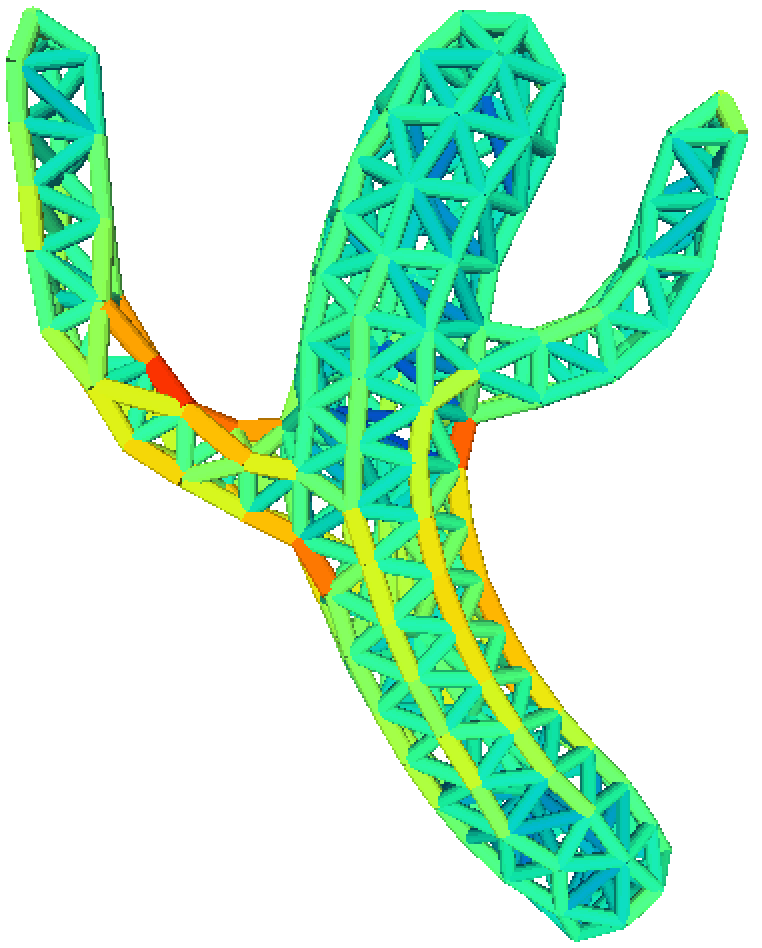
\includegraphics[width=.19\linewidth]{Figures/pipeline/3.png}
            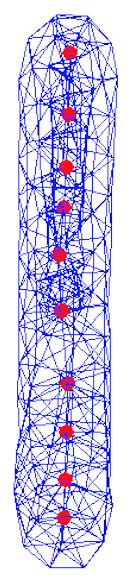
\includegraphics[width=.053\linewidth]{Figures/pipeline/m2.png}}\quad
    \subfigure[]{
            \label{fig:pipeline:d}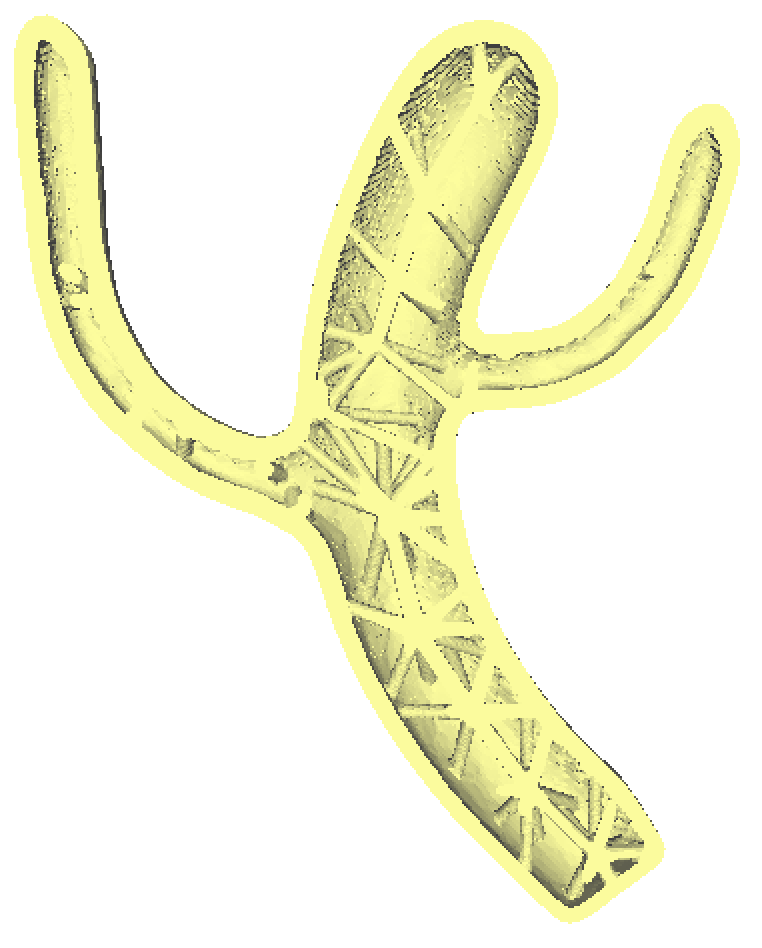
\includegraphics[width=.19\linewidth]{Figures/pipeline/4.png}}\quad

\caption{Pipeline of our approach. Given an input model (a), an initial frame structure (b) is generated. Our method runs a saddel point algorithm to obtain an optimized frame structure (c) which provides minimal deformation under unknown load distribution. (c) is colored to visualize their radii and a side view of the frame structure is presented to show the node position and topology connections before and after optimization. Then a post-processing step is applied to generate a solid structure (d) for 3D printing.
%
The front part of (d) is removed in order to show the internal structure.%Note that the beams in frame (c) have different radius and the shell of (d) is adaptive hollowed with different depth.
}
\label{fig:pipeline}
\end{figure*}



\noindent\textbf{Problem.}
The input of our framework is the surface mesh $S$.
%Assume the surface mesh $S$ of the input object is given.
Our goal is to generate an entity global stiffness object model $H$ consisting of an adaptive hollowed shell and a supportive interior sructure, while utilizing no more than a given amount of material. The generated object shares the same surface with as $S$ but has much less weight than $S$ for its lightweight supportive structure rather than solid filled.

\noindent\textbf{Remarks} The following two problems are usually considered in the structural optimization: Stiffness-to-Weight and Weight-to-Stiffness.
%%In the structural optimization field, researchers usually consider the following two problems:
Stiffness-to-Weight is to design a structure with the maximum stiffness using a specific amount of given material; and Weight-to-Stiffness is to design a structure with the least amount of material but satisfied the given stiffness expection. These two problems are dual and can be converted to each other by a simple binary search process. Without loss of generality, here we focus on the former one that takes the amount of material use as the constraint. We also consider the load is only from external forces as the internal forces, gravity for most of the time, remains very small compared with external forces so is ignored.



\subsection{Frame structure}
\label{subsec:frame}


%In the filed of fabrication engineering, an extensive attention has been paid to shape analysis and structural optimization [Crapo 1979; Crapo 1990; Rosenberg 1980; Haftka and Grandhi 1986].
%Many kinds of lightweight structures, including frame and honeycomb, have been developed to reduce weight and enforce strength~\cite{Kindinger:2001,wang:2013,buildtolast} during recent years.
%
%
%However, the vast majority of previous work focused on structural optimization and design under a given load environment like some specified forces.
%In real situation, an object might be handled or used in various possible ways, and specified forces cannot be exhaustive of all cases.
%As lacking of valid formulation for the above mentioned problem, traditional methods of structural optimization are unable to solve it efficiently.
%In this paper, the frame structure is proposed for not only being able to efficiently optimize but also formulating the adaptive hollowing and interior beams into a unified form.


%We adopt the frame structure~\cite{wang:2013} due to its ability of simulating the object, efficiency of optimizing the design, and the generation of the adaptive hollowing and interior lightweight supportive structure.
%The frame structure~\cite{wang:2013} is adopted here due to its ability to simulate the object, efficiently optimize the design, generate the adaptive hollowing and interior lightweight supportive structure into a unified form.



%formulating the adaptive hollowing surface shell and interior beams into a unified form as well as being able to efficiently optimize the design.
\parpic[r]{\label{fig:frame-structure}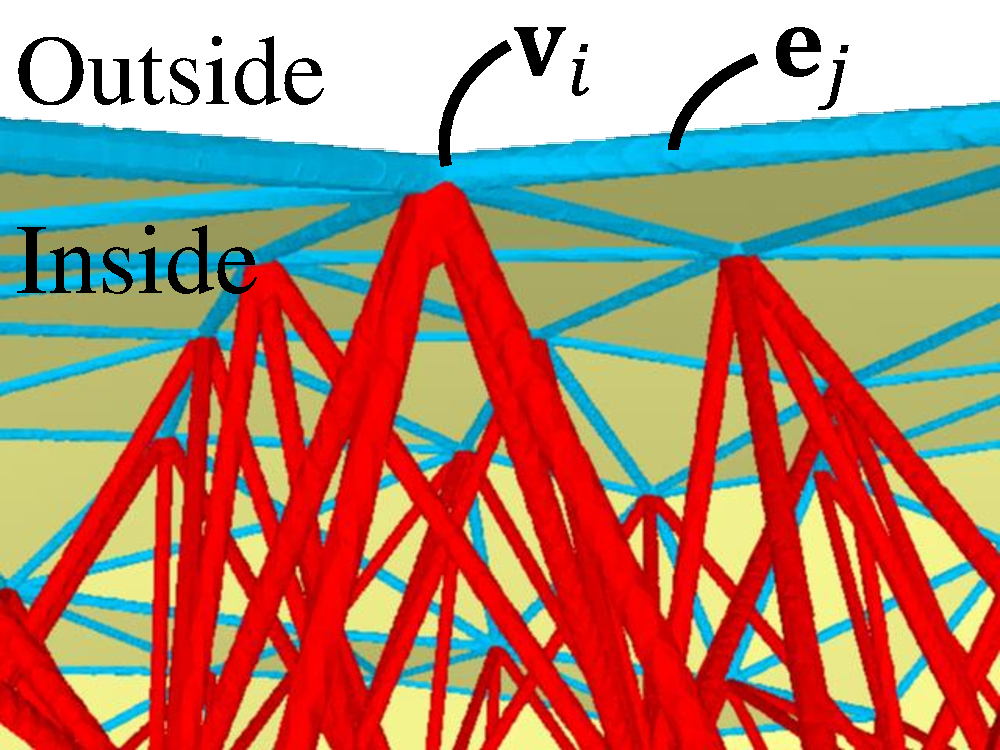
\includegraphics[width=0.2\linewidth]{Figures/structure/structure.pdf}}
%
A frame structure $\mathcal{T}$ consists of a set of frame nodes $V=\{\mathbf{v}_{i}, i=1,2,\cdots,m\}$ which are sampled on $S$ (marked in yellow) and in the volume enclosed by $S$, as well as a set of frame beams $E=\{\mathbf{e}_{j}, j=1,2,\cdots,n\}$ which are the edges connecting the nodes, as shown in the right figure.
%
Each node $\mathbf{v}_{i}$ represents a geometric position and each beam $\mathbf{e}_j$ is a cylindrical shape with radius $r_j$ and length $l_j$.
%
Here $\mathcal{T}$ can be seen as a graph of $V$ and $E$ with the geometry defining node positions, the beam radii, and the topology defining the connectivity between nodes.
%
For convenience, we also denote $V_S=\{\mathbf{v}_{i} \mid \mathbf{v}_{i}\in S\}$, $V_I=V\setminus V_S$,
$E_S=\{\mathbf{e}_j \mid \mathbf{e}_j\in S \}$ (marked in cyan), and $E_I = E\setminus E_S$ (marked in red).



%The frame structure~\cite{wang:2013} is adopted here due to formulating the adaptive hollowing surface shell and interior beams into a unified form
%as well as being able to efficiently optimize the design.
%%
%As shown in Figure~\ref{fig:frame-structure}\tuanfeng{a figure for frame structure}, a frame structure $\mathcal{T}$ consists of a set of frame nodes $V=\{\mathbf{v}_{i}, i=1,2,\cdots,m\}$ which are sampled on $S$ and in the volume enclosed by $S$, and a set of frame beams $E=\{\mathbf{e}_{j}, j=1,2,\cdots,n\}$ which are the edges connecting the nodes.
%%
%Each node represents a geometric position and each beam $\mathbf{e}_j \in E$ is a cylindrical shape with radius $r_j$ and length $l_j$.
%%
%Here $\mathcal{T}$ can be seen as a graph of $V$ and $E$ with the geometry defining node positions and beam radii, and the topology defining the connectivity between nodes.
%%
%For convenience, we also denote $V_S=\{\mathbf{v}_{i} \mid \mathbf{v}_{i}\in S\}$, $V_I=V\setminus V_S$,
%$E_S=\{\mathbf{e}_j \mid \mathbf{e}_j\in S \}$, and $E_I = E\setminus E_S$.



By taking adequate density of surface points, the appearance of frame $\mathcal{T}$ is expected to approximate $S$ within a certain geometric error \cite{yan2009isotropic}. After the frame is optimized, surface edges of frame (i.e., $E_S$) indicate the adaptive thickness (doubled radius) of the surface shell around the position of the edges.
Interior edges of the frame (i.e., $E_I$) are taken as cylinder-like supportive beams.
And then the frame $\mathcal{T}$ can be considered as a reasonable approximation of the final entity object $\mathcal{H}$.



%The frame structure is proposed for not only being able to efficiently optimize
%but also formulating the adaptive hollowing shell and interior beams into a unified form.



%Different from element-based methods for structural topology optimization where problems are expressed by element-wise step functions,
%the approach presented in this paper uses node positions and beam radii as design variables in the structural optimization.

The approach presented in this paper uses node positions and beam radii as design variables in the global stiffness structural optimization.
This is different from element-based methods for structural topology optimization~\cite{rozvany:2009}, where problems are expressed by tetrahedron-element-wise step functions.
%
As an effective discrete representation, the frame structure is fabrication-friendly and has simple mechanical properties which will be described in Section~\ref{subsec:mechanics}.



%
%\paragraph{Remark} When the optimization is finished, the optimized frame structure will guide on the solid generation. The interior structure is generated with a cylinder with the radii of an interior beam and the surface is adaptive hollowed with the depth equals to $\frac{2*(d_1*r_1+d_2*r_2+d_3*r_3)}{d_1+d_2+d_3}$, where $\{r_i,i=1,2,3\}$ is the radii of three most close beam with distance of $\{d_i,i=1,2,3\}$.
%


\subsection{Stiffness matrix}
\label{subsec:mechanics}


The mechanics of frame structure has been studied based on beam theory~\cite{Huges:1987,Gibson:1999,chandrupatla1991introduction} where frame beams are assumed to behave like simple beams under linear deformation caused by nodes' displacement or rotation. In our method, we make the following assumptions in calculating the equilibrium state of the structure.
\begin{itemize}
\item [a)] The beams are only connected to each other at nodes.
\item [b)] The beams are connected rigidly to have tensile, torsion, transverse shear force.
\item [c)] Each node has three displacement degrees of freedom and three rotation degrees of freedom.
\end{itemize}

\noindent\textbf{Linear relationship between deformation and force}
For a given frame structure, including both the surface and interior beams, the relationship between deformation \textemdash the displacement and rotation of each node, and the force (including torque) should satisfy the following discretized equilibrium equation.
\begin{equation} \label{eq:stiffness}
K(V,\mathbf{r}) D = F,
\end{equation}
where $V=(\mathbf{v}_1,\cdots,\mathbf{v}_m)$ also denotes the geometric positions of the nodes.
$K(V,\mathbf{r})$ is the stiffness matrix, which depends on node positions $V$ and beam radii $\mathbf{r}=(r_1,\cdots,r_n)$.
%
$F=(\mathbf{f}_1,\cdots,\mathbf{f}_m)^T$ is the force and torque distribution acting on each node and $D=(\mathbf{d}_1,\cdots,\mathbf{d}_m)^T$ is the displacement and the rotation of deformation caused by $F$.
For details, refer to~\cite{chandrupatla1991introduction}. Note that $F$ in Eq.~\eqref{eq:stiffness} is the sum of external force and only acts on a special set of nodes like $V_S$. This is for a better simulation of real world cases because external forces are always act on the surface.


\subsection{Eigen-Mode-like formulation}
%\subsection{Eigen-mode structural optimization}
\label{subsec:eigen-mode-opt}

Our global stiffness target, which minimizes the maximum deformation under unknown loads can be described as an Eigen-Mode-like formulation.

Originally, for the frame structure simulated from an object, we first find an external force $F$ that gives the maximal deformation. In order to avoid the scale problem, it is estimated by a deformation ratio $\frac{D^TD}{{F}^T{F}}$.
Then we minimize the maximal deformation ratio of the frame structure by varying the design variables $(V_I, \mathbf{r})$.


For an object in the state of equilibrium, the following conditions for $F$ are needed:
%
\begin{equation}
\label{cond-for-F}
\mathbf{1}\cdot F_i=0, \quad
 F_i \cdot (X_{i+1} -X_{c,i+1})-F_{i+1}\cdot (X_{i} -X_{c,i}) =0
\end{equation}
where $i=1,2,3$; $F_1,F_2,F_3$ are force components of $F$ along $x$, $y$, $z$ axis respectively; $X_1,X_2,X_3$
are the lists of $x$-, $y$-, $z$-coordinates of the nodes $X$ in a fame structure;
$X_{c}=(X_{c,1}, X_{c,2}, X_{c,3})$ is the center point of the object.
%
%\begin{equation}
%\label{cond-for-F}
%F_i = 0,\quad
% (F)_i \cdot (X_i -X_{c,i}) =0\quad (i=1,2,3)\:,
%\end{equation}
%where $\_1,\_2,\_3$ are force components along $x$, $y$, $z$ axis respectively; $X_1,X_2,X_3$
%are the lists of $x$-, $y$-, $z$-coordinates of the nodes $X$ in a fame structure;
%$X_{c}=(X_{c,1}, X_{c,2}, X_{c,3})$ is the centroid of the object. 
These two constrains indicate that both the force and the moment of the force are zero.
%As the upper bound of the amount of the material used is given, $G$ is a constant with two horizontal axis is zero.
%
%
%Also, for homogeneous Neumann boundary condition of $D$, the stiffness matrix
%$dK$ is singular. This is easy to seed since for a translation $D_0$ of object, $K D_0=0$.
%Moreover, let $R_0$ be the displacement vector from a rotation, we have $KR_0=0$.
%This fact also tells us that $\mbox{dim}(Null(K))=6$.
%
%
Since stiffness matrix $K$ is singular, for each $F$ satisfying Eq.~\eqref{cond-for-F}, to uniquely determine a solution $K D = F$, the translation and rotation should be ignored. Similiar to Eq.~\eqref{cond-for-F}, the total displacement and the total moment of displacement, the total rotation and the total moment of rotation are set to zero. Let the stiffness matrix under the above conditions on force and deformation be $\hat{K}$, which is now a regular matrix, then we have $D=\hat{K}^{-1}F$.
%

Thus, the structural optimization problem can be constructed as follows
\begin{equation} \label{eq:min-max-deformation}
\begin{array}{ccl}
\min\limits_{(V_I, \mathbf{r})\in\Theta} &
\max\limits_{F \mbox{ satisfying }  (\ref{cond-for-F}) } \frac{{(\hat{K}^{-1}F)}^T(\hat{K}^{-1}F)}{{F}^TF}
\end{array}
\end{equation}
where $\Theta$ is the collection of all feasible $V_I$ and $\mathbf{r}$; see detailed constrains in Sec.~\ref{subsec:constraints_for_opimization}.
%$$
%\min\limits_{(\mathbf{V}, \mathbf{r})\in\Theta}  \max \limits_{ \mathbf{1} \cdot F_i=0 } {(K^{-1}F)}^T(K^{-1}F)
%$$

\noindent\textbf{Eigen-Mode property} We here to discuss a more general situation if the external force can also act on $V_I$. As the stiffness matrix $\hat{K}$ is symmetric, the vector $F$ that maximizes the value ${{(\hat{K}^{-1}F)}^T(\hat{K}^{-1}F)}/{F^TF}$, accroding to \cite{Parlett:1998}, is just the eigenvector corresponding to the smallest eigenvalue of $\hat{K}$, denoted by $\lambda_{\min} (\hat{K})$ which is actually the same to the minimal positive eigenvalue of $K$.
%
Finally, we have such an eigen-mode optimization problem
\begin{equation}
\label{eq:max-min-eigenvalue}
\begin{array}{cl}
\max\limits_{(V_I, \mathbf{r})\in\Theta} & \lambda_{\min}^{*}(K(V,\mathbf{r}))
\end{array}
\end{equation}
where $\lambda_{\min}^{*}(K(V,\mathbf{r}))$ is the minimal positive eigenvalue of stiffness matrix $K(V,\mathbf{r})$.	


In this way, our formulation mathmatically proof the observation given by \cite{zhou:2013} that the eigenvector of kinematic equation indicates a structural worst-case. Here our linear relationship between deformation and force (ignored the first derivative of force) is a static but more realistic version of the kinematic equation. Our global stiffness optimization, therefore, can also be considered as automatically reinforce where the structure is the weakest. On the other hand, plenty of physical experiments done by \cite{zhou:2013} can also show that our deformation based formulation is reasonable in calculating 3D Printed object.


\subsection{ Constraints on structure design parameters}
\label{subsec:constraints_for_opimization}



\noindent\textbf{Radius bounds}
To make the frame structure printable, the radius of each beam should be no less than the minimum printable radius $\underline{r}$.
To avoid unrealistic design, an upper bound $\overline{r}$ for the radius is imposed for each beam.
Moreover, in order to retain the linear elastic property of the frame structure, the ratio between the length and the radius of a beam must satisfy the Euler buckling constraint.
%
In brief, the buckling and the printability can be integrated as a bounded constraint for each beam radius
\begin{equation} \label{eq:radius-bounds}
\underline{\eta}_j \leqslant {r}_j \leqslant \overline{r}, \quad  \mathbf{e}_j\in E,
\end{equation}
where $\underline{\eta}_j=\max(l_j/\alpha, \underline{r})$, $l_j$ is the length of beam $\mathbf{e}_j$, and $\alpha$ is the slenderness ratio.
%$\underline{r}$ is the minimum printable radius, and an upper bound $\overline{r}$.



%\if 0
%
%\paragraph{Buckling}
%%To validate the linear elastic property of frame, the ratio between the length and the radii of a beam should be constrained, which is known as Euler buckling and can be written as:
%%\begin{equation} \label{eq:buckling}
%%r_i \geqslant l_i / \alpha, \ \ \mathbf{e}_i \in E
%%\end{equation}
%%If the position of nodes are fixed, the buckling constrain can be considered as a lower buond of the radii of each beam.
%%
%In order not to fail the linear elastic property of frame structure,
%the ratio between length and radius of a beam must satisfy Euler buckling constraint
%\begin{equation} \label{eq:buckling}
%r_j \geqslant l_j / \alpha, \quad  \mathbf{e}_j \in E
%\end{equation}
%where $\alpha$ is the slenderness ratio.
%If the positions of nodes are fixed, the buckling constrain can be considered as a lower bound of the radius for each beam.
%
%\paragraph{Printability}
%To make the frame structure printable, the radius of each beam should be no less than the minimum printable radius $\underline{r}$.
%To avoid unrealistic design, we also set an upper bound $\overline{r}$ for each beam radius, i.e.,
%\begin{equation} \label{eq:printability}
%\underline{r}\leqslant {r}_j \leqslant \overline{r}, \quad  \mathbf{e}_j\in E.
%\end{equation}
%%
%%Note that both the buckling constraint and the printability constraint are imposed on the range of radius vector $\mathbf{r}$. For simplicity, we rewrite the constraint \eqref{eq:buckling} and \eqref{eq:printability} together as:
%%\begin{equation} \label{eq:lower_upper_r}
%%{r}_{j,lower} \leqslant {r}_j \leqslant {r}_{j,upper}, \quad \ \mathbf{e}_j\in E.
%%\end{equation}
%%where ${r}_{j,lower} = maximal(\underline{\eta},l_i / \alpha)$ and ${r}_{j,upper} = \overline{\eta}$.
%%
%For simplicity, the buckling~\eqref{eq:buckling} and the printability~\eqref{eq:printability} can be integrated into a range constraint of radius for each beam
%\begin{equation} \label{eq:radius-bounds}
%\underline{\eta}_j \leqslant {r}_j \leqslant \overline{r}, \quad  \mathbf{e}_j\in E.
%\end{equation}
%where $\underline{\eta}_j=\max(l_j/\alpha, \underline{r})$.
%
%\fi




\noindent\textbf{Volume}
%
The proposed problem is defined as optimizing the frame structure when a certain amount of material is given.
%
\parpic[r]{\label{fig:covered-area}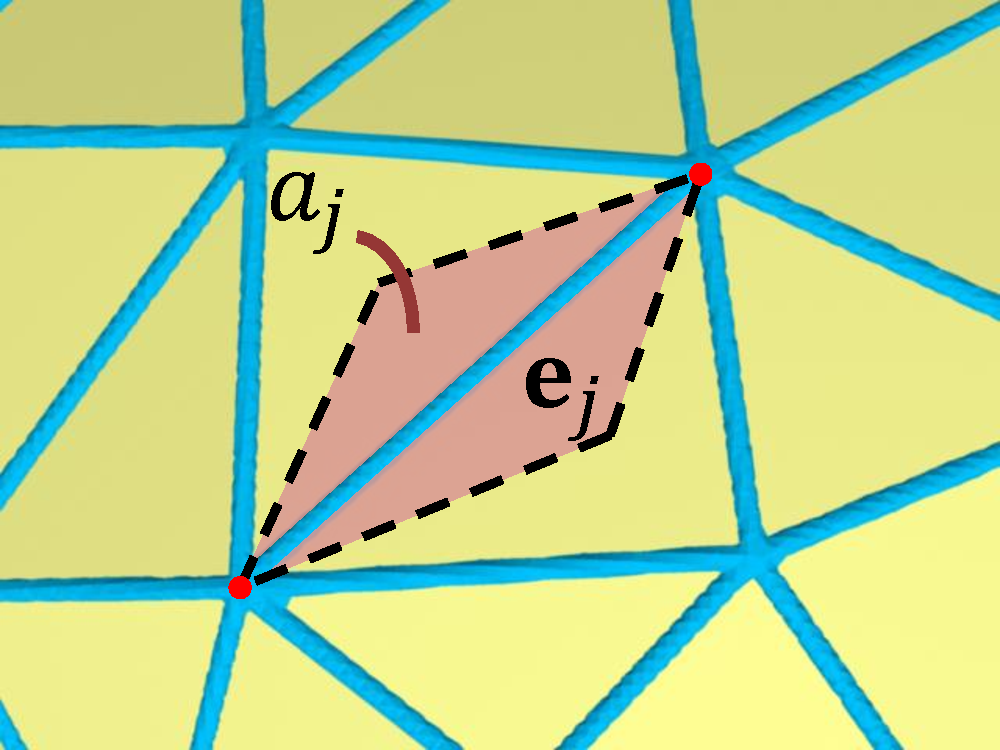
\includegraphics[width=0.2\linewidth]{Figures/area/area.pdf}}
Let $\overline{\mathrm{Vol}}$ be the amount of material available.
%Denote $\Omega$ the volume of solid material in designed structure $\mathcal{H}$.
%\parpic[r]{\label{fig:covered-area}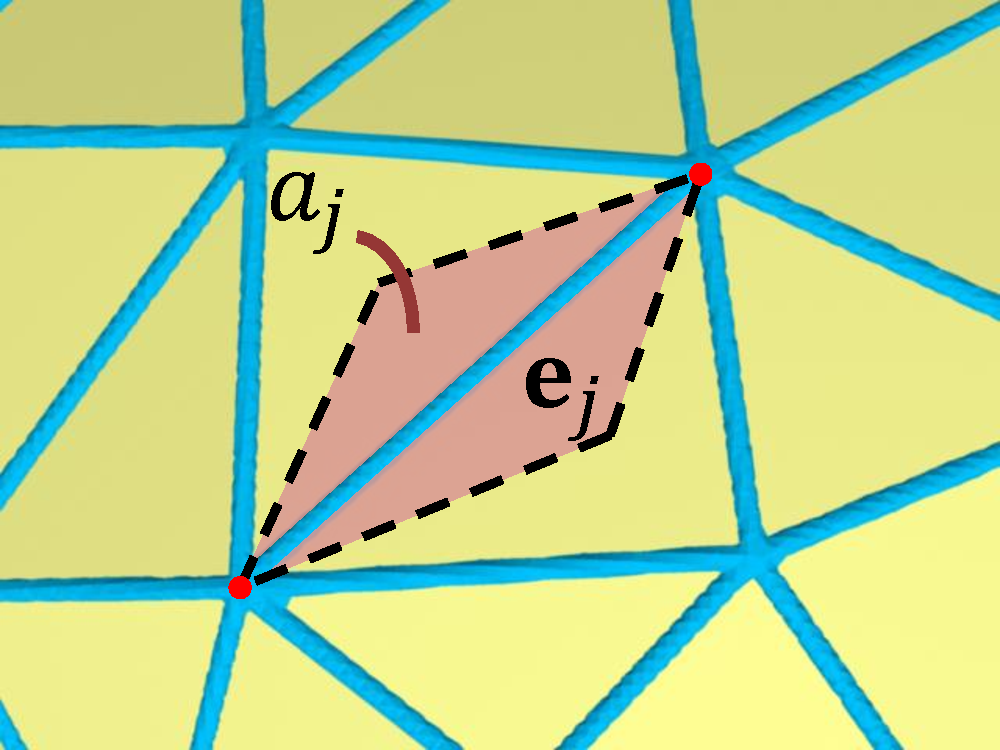
\includegraphics[width=0.4\linewidth]{Figures/area/area.pdf}}
The volume of solid material in the designed structure $\mathcal{H}$ consists of two parts:
the volume of interior beams in the frame, and the volume of adaptive-hollowed shell, which can be approximately calculated as
the sum of the product of the area covered by a surface beam and its doubled radius.
%
Thus we have a constraint on the material volume
\begin{equation} \label{eq:volume}
\sum_{\mathbf{e}_j\in E_I} \pi {r_j}^2 l_j + \sum_{\mathbf{e}_j\in E_S} 2 r_j a_j  \leqslant \overline{\mathrm{Vol}},
\end{equation}
where $a_j$ is the area covered by beam $\mathbf{e}_j$ on the surface.
In practice, $a_j$ is roughly calculated as the shaded area shown on the right.



%
%\[
%\Theta = \big\{ (\mathbf{V}, \mathbf{r}) \mid \ \mathrm{s.t.}\ \  \eqref{eq:radius-bounds}, \  \eqref{eq:volume} \big\}
%\]



%Overall, it's obvious that the most important constraint for the proposed problem is the total material cost, namely the volume upper bound $\overline{\Omega}$ of the solid $\mathcal{H}$.
%The volume of the solid consists of two parts: volume of interior structure, which is the same as the volume of interior beams of the frame, and the volume of adaptive-hollowed surface solid which can be approximately calculated as the sum of product of the area covered by a surface strframe edge 'covers' and doubled radii of the edge.\tuanfeng{figure}
%\begin{equation} \label{eq:volume}
%\sum_{\mathbf{e}_j\in E_1} \pi {r_i}^2 l_i + \sum_{\mathbf{e}_j\in E_2} 2r_i S_i  \leqslant \widetilde{\mathrm{Vol}}
%\end{equation}
%$S_i$ is the area which $i$th edge is coverd on the surface. In practice, we approximate $S_i$ with  $1/3$ of the are of the two triangles $\mathbf{e}_{i}$ attached.

\noindent\textbf{Shape barrier} The appearance of our optimal result should be the same with the surface of the input mesh. As a result, elements in internal beams set $E_I$ have to be kept inside of the volume enclosed by $S$. Many algorithms have been developed for this purpose. In our implementation, an efficient but approximate method is adapted that several test points are sampled from each beam for a quick check whether they are inside $S$. A feasable solution of the optimization problem is subject to the constraint that all the test points are inside $S$.



\noindent\textbf{Other constrains} The objective function of our optimization is very flexible and can be solved efficiently. As a result, addition constrains are able to be considered in our formulation such as stability, self-supportiveness, orientation, angle of beams, etc., including printability constrains specified by certain printing techniques. In this paper, we focus on the main problem \textendash \ global stiffness formulation, as these constrains have been well studied by many previous work~\cite{wang:2013}. 




%
%\begin{itemize}
%\item \textbf{Balance} For some standing objects, the center of mass of the output solid should be projected into the base of support\cite{prevost:2013}, which is easy to impose on the frame approximation with the same math form.
%\item \textbf{...}
%\end{itemize}




%
%
%\subsection{Eigen-mode structural optimization}
%\label{subsec:eigen-mode-opt}
%
%
%The problem at hand is defined as finding a frame structure which has the maximum global stiffness when a certain amount of material is given.
%In this section, we formulate the structural optimization problem that gives an optimal structure for all kind of force distribution by using eigen-mode analysis.
%For a frame structure of object, we first find a normalized  force $F$ (i.e., $\|F\|_{l^2}=1$) that maximizes
%the deformation $K^{-1}F$, which is estimated by $ \|K^{-1}F\|_{l^2} $.
%Then we optimize the maximal deformation of frame structure by varying the design variables $(V, \mathbf{r})$.
%
%Notice that since we are considering an equilibrium state, the following constraint conditions are needed:
%$$\mathbf{1}\cdot F_i=0,\quad (i=1,2,3)$$
%where $F=(F_1,F_2,F_3)$ are force components along $x, y, z$ coordinates respectively.
%Also, for homogeneous Dirichlet boundary condition of $D$, the stiffness matrix
%$K$ is singular, which is easy to see since for a translation $D_0$ of object, $K D_0=0$.
%This fact also tells us that $\mbox{dim}(Null(K))=3$. Thus, we append an constraint condition to $D$; for example,
%\begin{itemize}
%\item [a)] $\mathbf{1}\cdot  D=0$;
%\item [b)] $D=0$ for certain node.
%\end{itemize}
%With such a condition a) or b), there exists a unique $D$ for each $F$ that $\mathbf{1}\cdot F_i=0$ ($i=1,2,3$).
%In our model, to formulate an eigen-prolem, we choose the condition a).
%
%Since
%$(D+D_0)^T(D+D_0)=D^TD +D_0^TD_0$ for constant vector $D_0$, we know that each constraint condition of a) and b) gives the same shape of $D$, except for a shift, that maximizes $D^TD$.
%
%Thus, the structural optimization problem can be constructed as follows
%\begin{equation} \label{eq:min-max-deformation}
%\begin{array}{ccl}
%\min\limits_{(V, \mathbf{r})\in\Theta} &
%\max\limits_{\mathbf{1}\cdot F_i=0} {(K^{-1}F)}^T(K^{-1}F)
%\end{array}
%\end{equation}
%where $\Theta=\big\{(V, \mathbf{r}) \mid \ \text{subject to}\  \eqref{eq:radius-bounds} \ \text{and}\  \eqref{eq:volume}\big\}$.
%%$$
%%\min\limits_{(\mathbf{V}, \mathbf{r})\in\Theta}  \max \limits_{ \mathbf{1} \cdot F_i=0 } {(K^{-1}F)}^T(K^{-1}F)
%%$$
%Notice that the vector $F$ that maximizes the value  ${(K^{-1}F)}^T(K^{-1}F)$ is just the eigenvector
%corresponding to the largest eigenvalue of $K^{-T}K^{-1}$, denoted by $\lambda_{\max}(K^{-T}K^{-1})$.
%As $K$ is a symmetric matrix, $K^{-T}K^{-1}$ and $K$ have the same eigenvectors and the relationship of their eigenvalues by
%$$
%\lambda(K^{-T}K^{-1})=\dfrac{1}{\lambda(K)^2}.
%$$
%%Moreover, the eigenvector of $K$ with the constraint $a)$ or $b)$ is just the non-constant eigenvecotr of $K$ without constraint conditions.
%Thus, the force vector that maximizes ${(K^{-1}F)}^T(K^{-1}F)$ is given by the eigenvector of matrix $K$ corresponding to its smallest eigenvalue, denoted by $\lambda_{\min} (K)$, and reaches the maximum value of objective function as $\lambda_{\max}(K^{-T}K^{-1})=1/{\lambda_{\min}(K)^2}$.
%
%In practical computation, we can construct the stiffness matrix without constraint condition for $D$ and $F$ to
%obtain $\hat{K}$. Then, it is easy to see that the $\lambda_{\min} (K)$ is the minimal positive eigenvalue of $\hat{K}$.
%
%
%As a summary, we have such an eigen-mode optimization problem
%%$$
%%\max\limits_{(\mathbf{V}, \mathbf{r})\in\Theta}   \lambda_{\min} (K)
%%$$
%\begin{equation}
%\label{eq:max-min-eigenvalue}
%\begin{array}{cl}
%\max\limits_{(V, \mathbf{r})\in\Theta} & \lambda_{\min}^{*}(K(V,\mathbf{r}))
%\end{array}
%\end{equation}
%where $\lambda_{\min}^{*}(K(V,\mathbf{r}))$ is the minimal positive eigenvalue of stiffness matrix $K(V,\mathbf{r})$.
%


%\xuefeng{My revision ends here.}

%
%
%The problem at hand is defined as finding an almighty frame structure which has the maximum global stiffness
%under any unprescribed loads when a certain amount of material is given.
%%
%A frame structure with maximum global stiffness provides a minimum mean compliance for the worst-case (most-damaged) loads.
%%A frame structure with maximum global stiffness provides a minimum for the external work with the real displacement field or minimum mean compliance.
%%
%Since minimization of mean compliance is equivalent to the maximization of the total potential energy,
%the almighty structural optimization problem can be constructed as follows
%%(Hassani and Hinton 1999; Bendsoe and Sigmund 2003)%
%%
%\begin{equation} \label{eq:min-max-deformation}
%\begin{array}{ccl}
%\max\limits_{(\mathbf{V}, \mathbf{r})\in\Theta} &
%\min\limits_{\mathbf{D}\in\Pi} & \mathbf{D}^T \mathbf{K}(\mathbf{V},\mathbf{r})\mathbf{D}
%\end{array}
%\end{equation}
%where $\mathbf{D}\in\Pi = \big\{ \mathbf{D} \mid   \|\mathbf{D}\|_2=1,\sum\limits_{i=1}^m \mathbf{d}_i =\mathbf{0},\sum\limits_{i=1}^m \mathbf{v}_i\times\mathbf{d}_i =\mathbf{0} \big\}$ is the real displacement field,
%$\mathbf{D}^T \mathbf{K}(\mathbf{V},\mathbf{r})\mathbf{D}$ is total potential energy,
%and $(\mathbf{V},\mathbf{r})\in\Theta=\big\{(\mathbf{V}, \mathbf{r}) \mid \ \text{subject to}\  \eqref{eq:radius-bounds} \ \text{and}\  \eqref{eq:volume}\big\}$ are design variables in the frame structure.
%%
%Note that minimization of the total potential energy in~\eqref{eq:potential-energy-max} according to constrained $\mathbf{D}$
%is equivalent to satisfying the state equilibrium.
%%
%In the almighty structural optimization, the goal can be thought of as determination of optimal design variables
%to achieve the best load-bearing performance under any possible deformation.
%
%
%%\[
%%\Pi = \big\{ \mathbf{D} \mid   \|\mathbf{D}\|_2=1,
%%\sum\limits_{i=1}^m \mathbf{d}_i =\mathbf{0},\sum\limits_{i=1}^m \mathbf{v}_i\times\mathbf{d}_i =\mathbf{0} \big\}
%%\]
%%
%%\[
%%\Theta = \big\{ (\mathbf{V}, \mathbf{r}) \mid \ \text{subject to}\  \eqref{eq:radius-bounds} \ \text{and}\  \eqref{eq:volume} \big\}
%%\]
%
%
%
%In fact, the stiffness matrix $\mathbf{K}(\mathbf{V},\mathbf{r})$ is positive-semidefinite.
%The optimization of~\eqref{eq:potential-energy-max} can be reformulated as to maximizing the minimum non-zero eigenvalue of stiffness matrix, i.e.,
%\begin{equation}
%\label{eq:max-min-eigenvalue}
%\begin{array}{cl}
%\max\limits_{(\mathbf{V}, \mathbf{r})\in\Theta} & \lambda_{\min}^{*}(\mathbf{K}(\mathbf{V},\mathbf{r}))
%\end{array}
%\end{equation}
%where $\lambda_{\min}^{*}(\mathbf{K}(\mathbf{V},\mathbf{r}))$ represents the minimum non-zero eigenvalue of $\mathbf{K}(\mathbf{V},\mathbf{r})$.
%%
%Note that the constraints of deformation displacement field $\mathbf{D}$ have been implicitly passed on to the minimum non-zero eigenvalue of stiffness matrix.



\section{Methodology}
\label{sec:algorithm}

%When an object mesh is given, instead of optimize the inside solid distribution, we simulate the whole structure via frame and optimize the frame parameter respectively. In this section, we will give a detailed description on how to generate an initial frame structure from a given mesh, optimization techniques and a solid-generation process to encode the frame parameter back to a 3D PLC mesh for fabrication.

We propose a novel approach based on the formulation Eq.~\eqref{eq:min-max-deformation} to find a global stiffness structure
which provides the best load-bearing performance under any possible load distributions.
%
An overview of our algorithm is shown in Figure~\ref{fig:pipeline}.
%
Given a closed 3D input surface $S$ represented by a triangular mesh, we first compute an isotropic initial frame with its beams of lower bound radii. We use the \emph{Constrained Centroidal Voronoi Tessellation}~(CCVT)~\cite{Yan:2010} for this step (see Figure~\ref{fig:pipeline}(b) for an example).
%
Starting from this initial frame, we then iteratively optimize the beam radii and node position by solving a saddle point problem (see Figure~\ref{fig:pipeline}(c)), to achieve a frame with maximum global stiffness under the volume constraint.
%
Finally, we apply a post-processing step to the optimized frame structure to generate an entity object that inherits the global stiffness property as the final result (see Figure~\ref{fig:pipeline}(d)).


\subsection{Frame initialization}
\label{subsec:initialization}


We choose an isotropic tetrahedralization approach~\cite{Yan:2010} to guide the frame initialization, with a uniform density function, for our purpose.
We first randomly generate a set of sites in the interior domain of surface $S$.
The number of sites is specified by the user, it is related to the complexity of frame structure. Then we minimize the CCVT energy function by iteratively optimizing the positions of the sites.
Once the optimization is terminated, the dual triangulation is extracted as the initial frame.
This initial frame will be determined by having each tetrahedral edge as a frame beam with the radius $\underline{\eta}$ (defined in Eq.~\eqref{eq:radius-bounds}). Although an adaptive initialization is considered to benefit the start point of optimization, it is actually ill-posed as our target is to strengthen the weakest. If the initialization is adaptive to the initial weakest situation, it will no longer benefit the final result as the weakest situaiton is changing during the optimization (see Fig.~\ref{fig_frame_max}). On the other hand, an isotropic initialization is good enough as our geometry optimization is shown to contributed a lot to the final result (see Fig.~\ref{fig:pipeline:d}).



%\paragraph{Adaptive initialization dilemma}
%It is obvious that the load-bearing performance is related to the geometry of the surface $S$.
%A good structure design should then rely on the geometry information.
%However, adaptive initialization is not a good option since it might become inappropriate after some iterations of optimization.
%The reason is that the stage result of optimization might change the easy-damaged place and might lead to the adaptive initialization turning into restraint of further optimization.
%As a consequence, we perform a uniform density function when computing the CCVT on the given mesh $S$.


\noindent\textbf{Remarks}
For thin details on the surface, damage can easily happen even without any hollowing.
So as a part of the initialization, we first simplify all the thin parts and add these geometric details back only after the solid object is finally generated.
This is automatically realized thanks to the natural limitation of CCVT, which eliminates thin parts by optimizing the energy function with a uniform density function.



\subsection{Saddle point algorithm}
%\subsection{Saddle point algorithm}
\label{subsec:opt-algorithm}


%\tofix{This section describe the algorithm for solving the optimization problem. and topology clean is also mentioned}



In global stiffness structural optimization~\eqref{eq:min-max-deformation}, derivatives of the objective function, e.g., gradients, with respect to $V_I$ and $\mathbf{r}$ cannot be explicitly expressed and efficiently calculated.
%
It would be extremely unfavorable to employ most iterative strategies that make use of the first and probably second derivatives of the objective function.
%While the computational cost of direct search method without using gradient information would be too expensive and very time-consuming.
However, without using gradient information, the computational cost of using direct search methods would be too expensive and too time-consuming.
%
Through rigorous mathematical derivation, we will present an algorithm based on the Rayleigh-quotient to greatly accelerate the solving of the problem.





We first define the Rayleigh-quotient~\cite{Parlett:1998} of the stiffness matrix $K(V,\mathbf{r})$ as
\begin{equation} \label{eq:rayleigh-quotient}
Q(V, \mathbf{r}, \mathbf{u})=\dfrac{<K( V  ,\mathbf{r})\mathbf{u},\mathbf{u}>}{<\mathbf{u},\mathbf{u}>}.
\end{equation}
According to the extremal property of Rayleigh quotient, the global stiffness structural optimization~\eqref{eq:min-max-deformation} is equivalent to the following saddle point problem
\begin{equation}\label{eq:max-min-Rayleigh}
\begin{array}{ccl}
\max\limits_{(V_I,\mathbf{r})\in\Theta} & \min\limits_{\mathbf{u}\in N(K)^{\perp}} & Q(V, \mathbf{r}, \mathbf{u})
\end{array}
\end{equation}
where $N(K)^{\perp}=\{\mathbf{u} \mid \mathbf{z}_i^T \mathbf{u}=0, i=1,\cdots,6\}$ is the orthogonal complement of
$Null(K)=\mathrm{span}\{\mathbf{z}_1,\cdots,\mathbf{z}_6\}$.
In the saddle point problem~\eqref{eq:max-min-Rayleigh}, the gradients $\{\nabla_{V} Q, \nabla_{\mathbf{r}} Q, \nabla_{\mathbf{u}} Q\}$
have explicit expressions and can be computed efficiently.
Thus, we can design a Rayleigh-quotient based algorithm for optimizing the frame structure as follows.



\begin{algorithm}[!htb]
\textbf{Input:} an initial frame $\mathcal{T}^{(0)}$ obtained in Section~\ref{subsec:initialization}  \\
\textbf{Output:} an optimized frame $\mathcal{T}$ with its design variables $(V_I,\mathbf{r})$ \\

\begin{algorithmic}

	\STATE \textbf{Step 1:} Get $(V^{(0)},\mathbf{r}^{(0)})$ from the initial frame,
    obtain the eigenvector $\tilde{\mathbf{u}}^{(0)}$ corresponding to the minimal positive eigenvalue of $K(V^{(0)},\mathbf{r}^{(0)})$, 
    %$=\arg\min\limits_{\mathbf{u}\in N(K)^{\perp}}Q(V^{(0)}, \mathbf{r}^{(0)}, \mathbf{u})$,
    specify a threshold $\epsilon$, and let $k:=1$.

    \STATE \textbf{Step 2:} Update $(V_I^{(k)},\mathbf{r}^{(k)})=\arg\max\limits_{(V_I,\mathbf{r})\in\Theta}Q(V, \mathbf{r}, \tilde{\mathbf{u}}^{(k-1)})$ by the interior-point algorithm~\cite[Chapter~19]{Nocedal:2006}.

    \STATE \textbf{Step 3:} 
    Compute the minimal positive eigenvalue of $K(V^{(k)},\mathbf{r}^{(k)})$ and its corresponding eigenvector $\tilde{\mathbf{u}}^{(k)}$.
    %Solve the linear equality-constrained optimization
    %$\tilde{\mathbf{u}}^{(k)}=\arg\min\limits_{\mathbf{u}\in N(K)^{\perp}}Q(V^{(k)}, \mathbf{r}^{(k)}, \mathbf{u})$ using Lagrange-Newton method.

    %% Compute null subspace of $K$, $Null(K(V^{(k)},\mathbf{r}^{(k)}))$

    \STATE \textbf{Step 4:} If $Q(V^{(k)},\mathbf{r}^{(k)},\tilde{\mathbf{u}}^{(k)})-Q(V^{(k-1)},\mathbf{r}^{(k-1)},\tilde{\mathbf{u}}^{(k-1)}) \leq \epsilon$,
    then output $(V^{(k)},\mathbf{r}^{(k)})$ as optimized design variables for the final frame;
    Otherwise, go back to \textbf{Step 2}.

\end{algorithmic}
\caption{Rayleigh-quotient based algorithm} \label{alg:Rayleigh-quotient-algorithm}
\end{algorithm}




When the optimized frame is generated from our Rayleigh-quotient based algorithm,
we will then merge any pairs of nodes that are connected by a strut that is at the minimum allowable length.
The struts with small radii can also be eliminated to simplify the structure by applying a sparse optimization described in~\cite{wang:2013}.
After this topology-cleaning step, we will use the optimized frame to generate a solid structure $\mathcal{H}$ for 3D printing.






\subsection{Postprocess}
\label{subsec:post-processing}


The ultimate goal of our approach is to generate an entity object $H$ inside the surface boundary $S$.
For this purpose, we separate the optimized frame $\mathcal{T}$ into the boundary beam set $E_S$ and the interior beam set $E_I$, as discussed in Section~\ref{subsec:frame}. The beam sets $E_S$ and $E_I$ will guide the adaptive hollowing and interior structure generation, respectively.

First, the radii of the surface beams are used to determined a thickness function as
\[
\zeta(\mathbf{p})= 2(w_1 \cdot r_{j_1} + w_2 \cdot r_{j_2} + w_3 \cdot r_{j_3}), \  \forall \mathbf{p}\in S,
\]
where $\{r_{j_1},r_{j_2},r_{j_3}\}$ are the radii of three surface beams from triangle $\triangle \mathbf{e}_{j_1}\mathbf{e}_{j_2}\mathbf{e}_{j_3}\subset E_S$ where the point $\mathbf{p}$ lies, and $\{w_1,w_2,w_3\}$ are its barycenter coordinates.
%
Let $\Omega\subset\mathbb{R}^3$ be the region bounded by the input surface mesh $S$.
%
Then the adaptive hollowed surface shell is defined as
\begin{equation} \label{eq:adaptive-shell}
H_S=\{\mathbf{q}\in\Omega \mid \|\mathbf{q}-\mathbf{p}\| \leqslant \zeta(\mathbf{p}), \ \forall\mathbf{p}\in S \},
\end{equation}
which can be considered as a piecewise linear interpolation of the surface beams $E_S$.
%
Similarly, the beams in $E_I$ are used to define the interior supportive structure as
\begin{equation} \label{eq:interior-structure}
H_I=\{\mathbf{q}\in\Omega \mid \mathrm{dist}(\mathbf{q}, \mathbf{e}_j) \leqslant r_j, \ \forall\mathbf{e}_j\in E_I \},
\end{equation}
where $\mathrm{dist}(\mathbf{q}, \mathbf{e}_j)$ is the geometric distance of point $\mathbf{q}$ to the line segment $\mathbf{e}_j$.
%
The whole solid structure $H$ can then be given as
\[
H = H_S \bigcup H_I.
\]
Finally, we apply the \emph{Extended Dual Contouring} (EDC) algorithm~\cite{cwang:2013} to extract the 2-manifold surface boundary of solid $H$.
%
As shown in Figure~\ref{fig:pipeline}(d), the generated solid structure with its boundary mesh is now ready for 3D printing.




%As the ultimate goal here is to generate a solid structure $\mathcal{H}$ within the surface $S$, we seperate the generated frame $\mathcal{T}$ into surface beam set $E_1$ and interior beam set $E_2$ as discussed in section\ref{frame} and guide the adaptive hollwing and interior structure generation, respectivly. We first define the distance of a point to the surface $S$ as
%\begin{equation} \label{eq:dist}
%dist(\mathbf{p},S)=\inf_{\forall \mathbf{q} \in S} \parallel \mathbf{p-q} \parallel,
%\end{equation}
%and for adaptive hollowing, a depth $d_\mathbf{p}$ should be defined on point $\mathbf{p}$ on surface $S$ as well. The adaptive hollowed solid is then defined as:
%\begin{equation} \label{eq:adaptive_hollowing}
%\mathcal{H}_1=\{\mathbf{q} \ in \  S \mid \exists \mathbf{p} \  on \ S, d_{\mathbf{p}} \geqslant \parallel \mathbf{pq} \parallel\}.
%\end{equation}
%As the radius of frame beams in $E_1$ can help on determining the depth of a place on $S$, we set
%\begin{equation} \label{eq:depth}
%d_{\mathbf{p}}= 2\frac{r_1*d_1+r_2*d_2+r_3*d_3}{d_1+d_2+d_3},
%\end{equation}
%where $r_i$ is the radii of three closest beams in $E_1$ with distance of $d_i$. In other words, the depth of surface can be considered as an interpolation of three most close surface frame beams. Meanwhile, beams in $E_2$ are used to generate interior structure as
%\begin{equation} \label{eq:interior_structure}
%\mathcal{H}_2=\{\mathbf{q} \ in \  S \mid \exists \mathbf{e}_i \in E_2 , dist^*(\mathbf{q},\mathbf{e}_i)<r_i\}.
%\end{equation}
%where $dist^*$ is the distance between point and line segment.
%
%After adding cylinder-like structure guided by beams in $E_2$, the whole solid $\mathcal{H}$ can be defined as:
%\begin{equation} \label{eq:solidgen}
%\mathcal{H} = \mathcal{H}_1 \bigcup \mathcal{H}_2.
%\end{equation}
%Applying an extended dual contouring (DC) algorithm discribed in \cite{cwang:2013}, we generate solid with 2-manifold surface(both outside and inside) which is suitable for 3D printing.






\section{Results and discussion}
\label{sec:result}

In this section, we present some computational results of the proposed approach. Our approach offers a global stiffness design of interior structure with the input surface mesh and the amount of material allowed. Our algorithm is applied to a variety of objects that would be applied with different load distributions in regular use like American football, toys and models. We first verify the optimization results of our formulation with the analysis framework in Sec.~\ref{subsec:mechanics}, and then verify the final results of the whole framework which are generated based on the optimized frame structures. Different from verifying the result of optimization under given load, our global stiffness optimization result is difficult to test in real physical experiment but thanks to the advance of FEM technique, we examed our results based on a FEM-based computational framework that can be considered as a good simulation of physical experiment, which will be discussed later. 

\noindent\textbf{Criteria} With a $10N$ load is applied, two criteria are discussed here: \textit{Average} deformation and \textit{Maximum} deformation. $4000$ random load distribution cases are applied and the \textit{Average} is the mean value of the norm of the $4000$ deformation led by corresponding load distributions. \textit{Maximum} is obtained by applying the load that leads to the maximum norm of deformation: on frame structure, the load distribution is given by the inner optimization of our formulation, i.e., $\max\limits_{F \mbox{ satisfying }  (\ref{cond-for-F}) } \frac{{(\hat{K}^{-1}F)}^T(\hat{K}^{-1}F)}{{F}^TF}$; on the final object, the load distribution is given by the result of \cite{zhou:2013}. In our experiment, the amount of material use is set to be the $20\%$ of the solid volume of the input object. A better global stiffness property means the less value these two criteria are. 

All the experiments were conducted on a PC with a 2.8GHZ Core CPU and 8GB RAM, running Linux OS.

To verify the global stiffness property of our optimized frame structure, we compare it and the initial structure with uniform beam radii. The uniform radii is set to make the control structure have the same volume as our result. In Fig.~\ref{fig_frame_hand_case}, two certain cases of the hand model is presented where warmer color refers to a larger value of deformation and cooler color refers to a smaller value of deformation. For all the tested models, the map of the \textit{Maximum} deformation is illustrated in Fig.~\ref{fig_frame_max}. With the statistic data in Table~\ref{table_frame}, our proposed formulation is proved to be able to optimize the global stiffness of a given initial frame structure.


\begin{figure}[h]
  \centering
  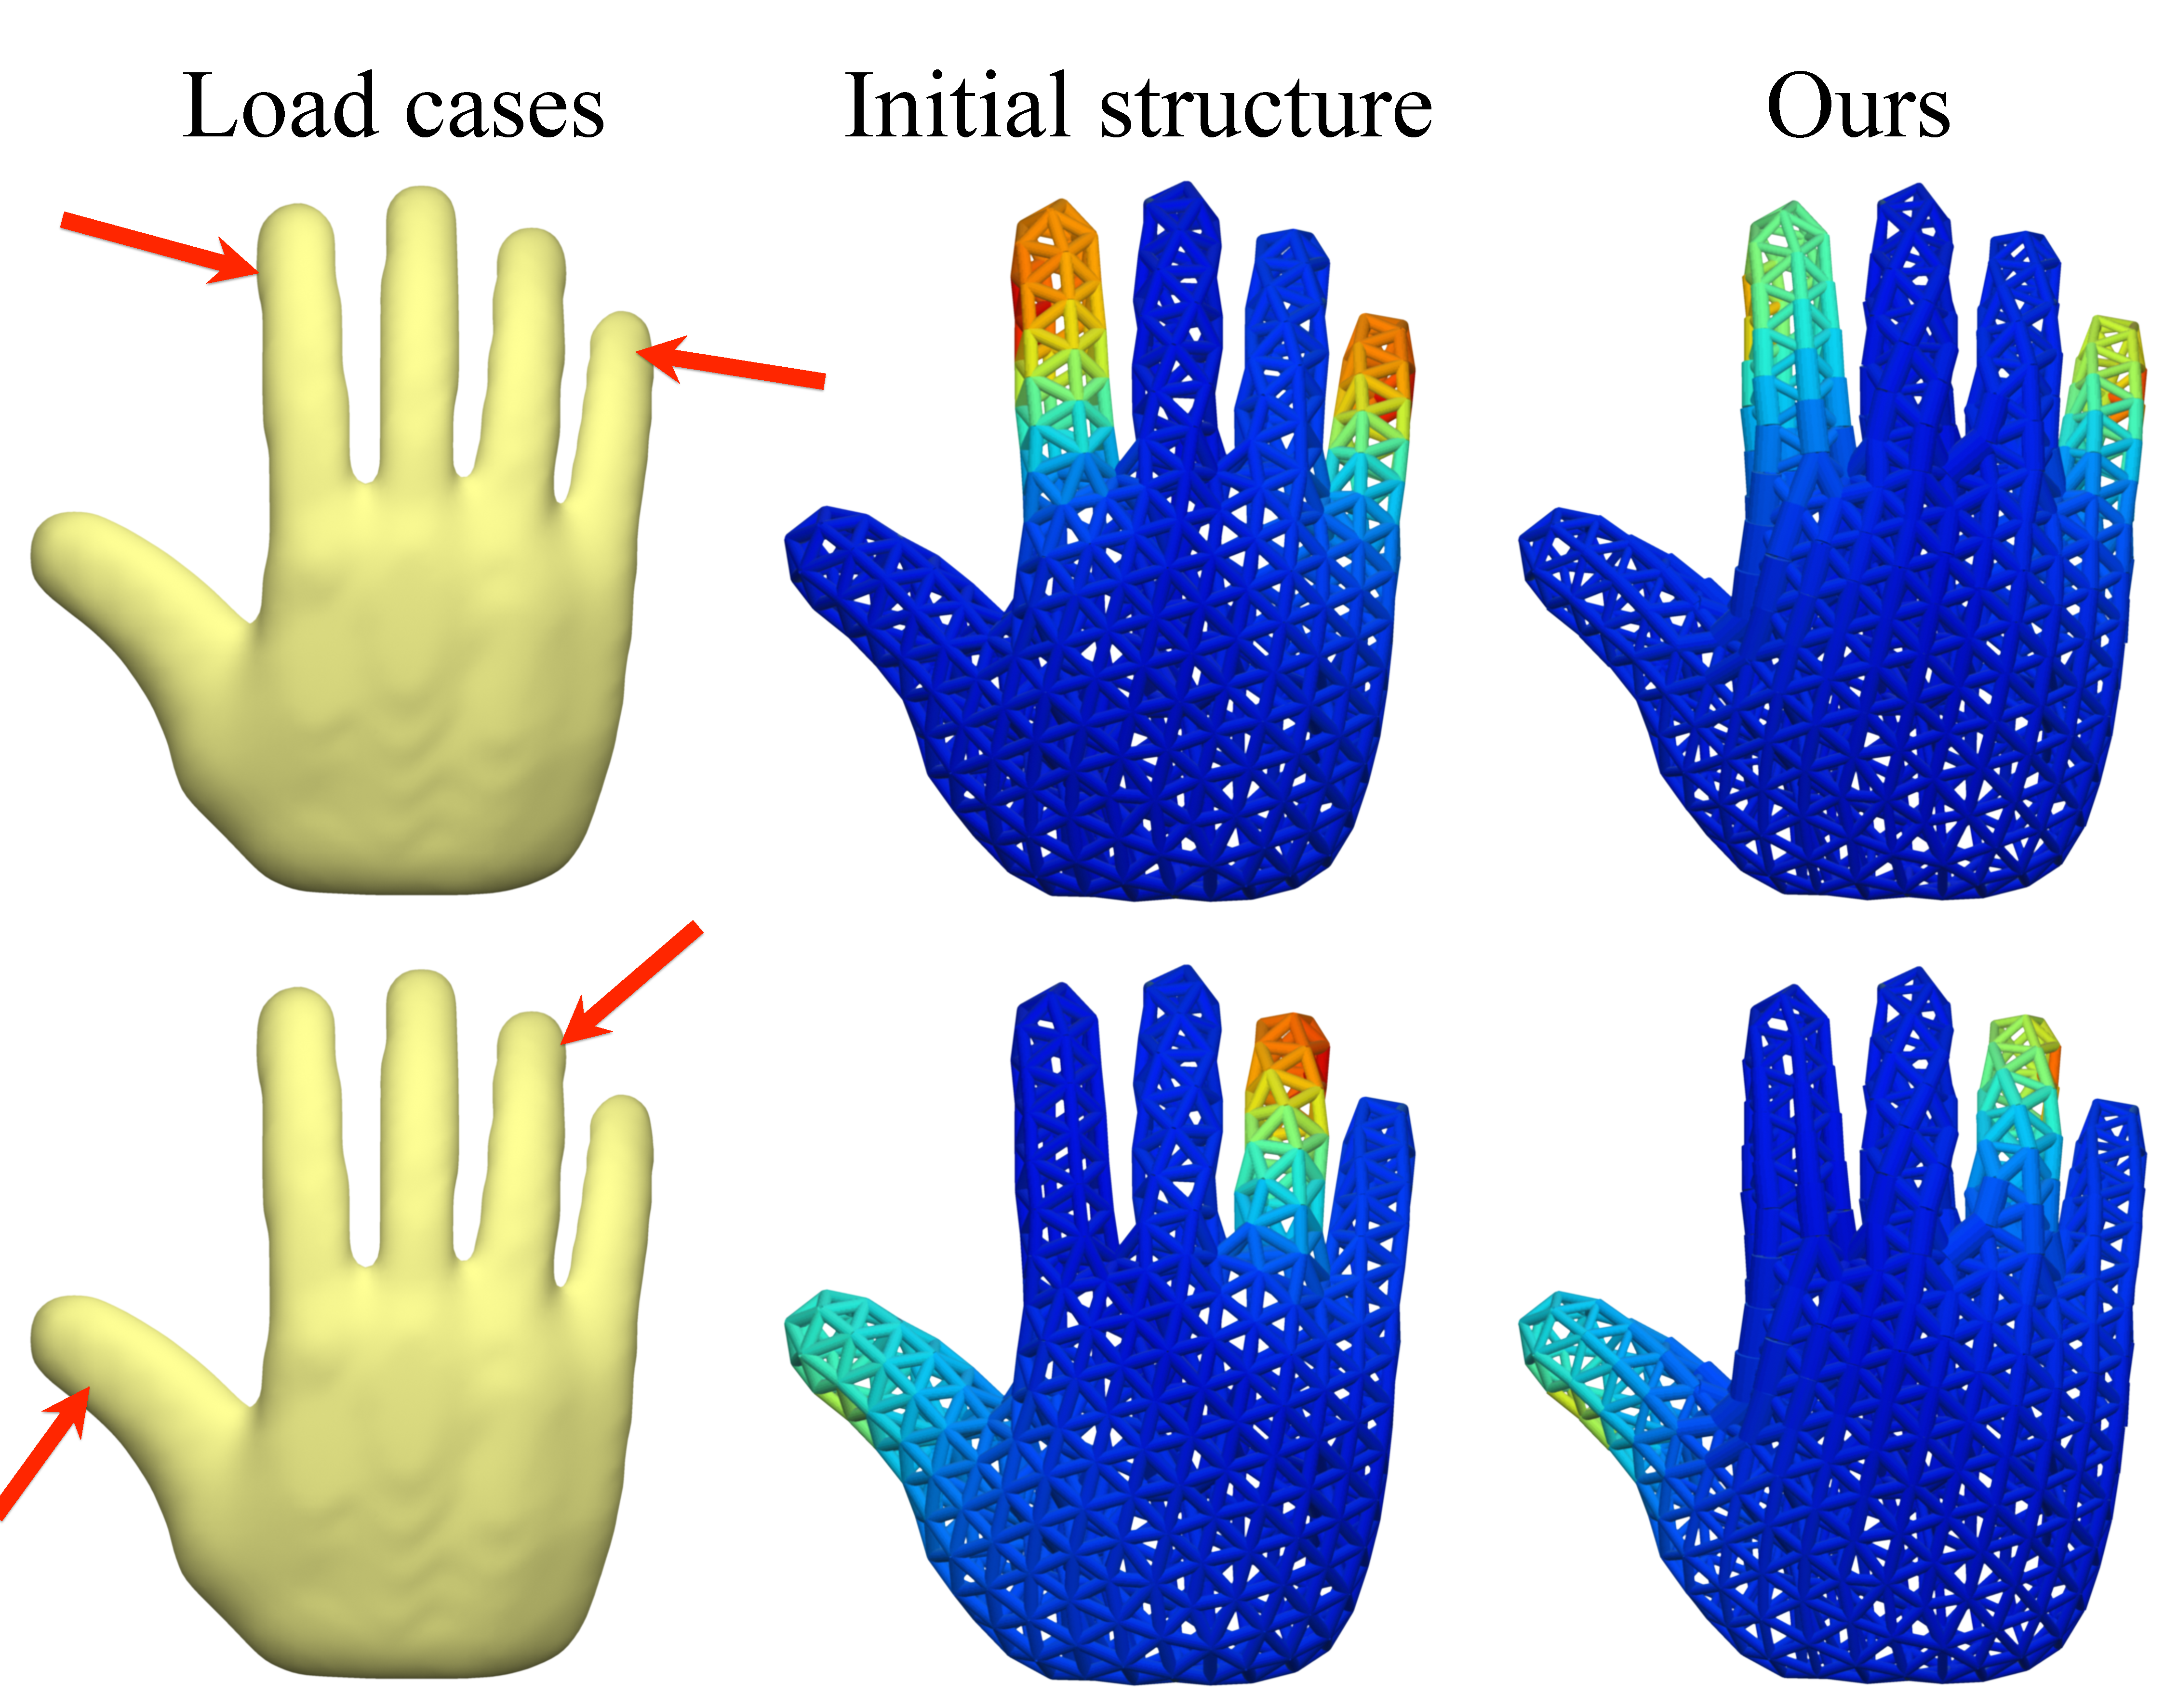
\includegraphics[width=0.5\linewidth]{Figures/hand/hand.pdf}
  \caption{\label{fig_frame_hand_case} Deformation distribution of two certain load distribution cases (top and bottom row) on the initial structure and our optimized structure of hand model. The red arrows shown on the model indicate that the deformation is simulated under the certain pair of forces. The initial structure we tested have the same volume with our result. Warmer color refers to a larger value of deformation and cooler color refers to a smaller value of deformation. It is obvious that our result performs better in these two selected cases.}
\end{figure}

\begin{figure*}[t]

  \centering
            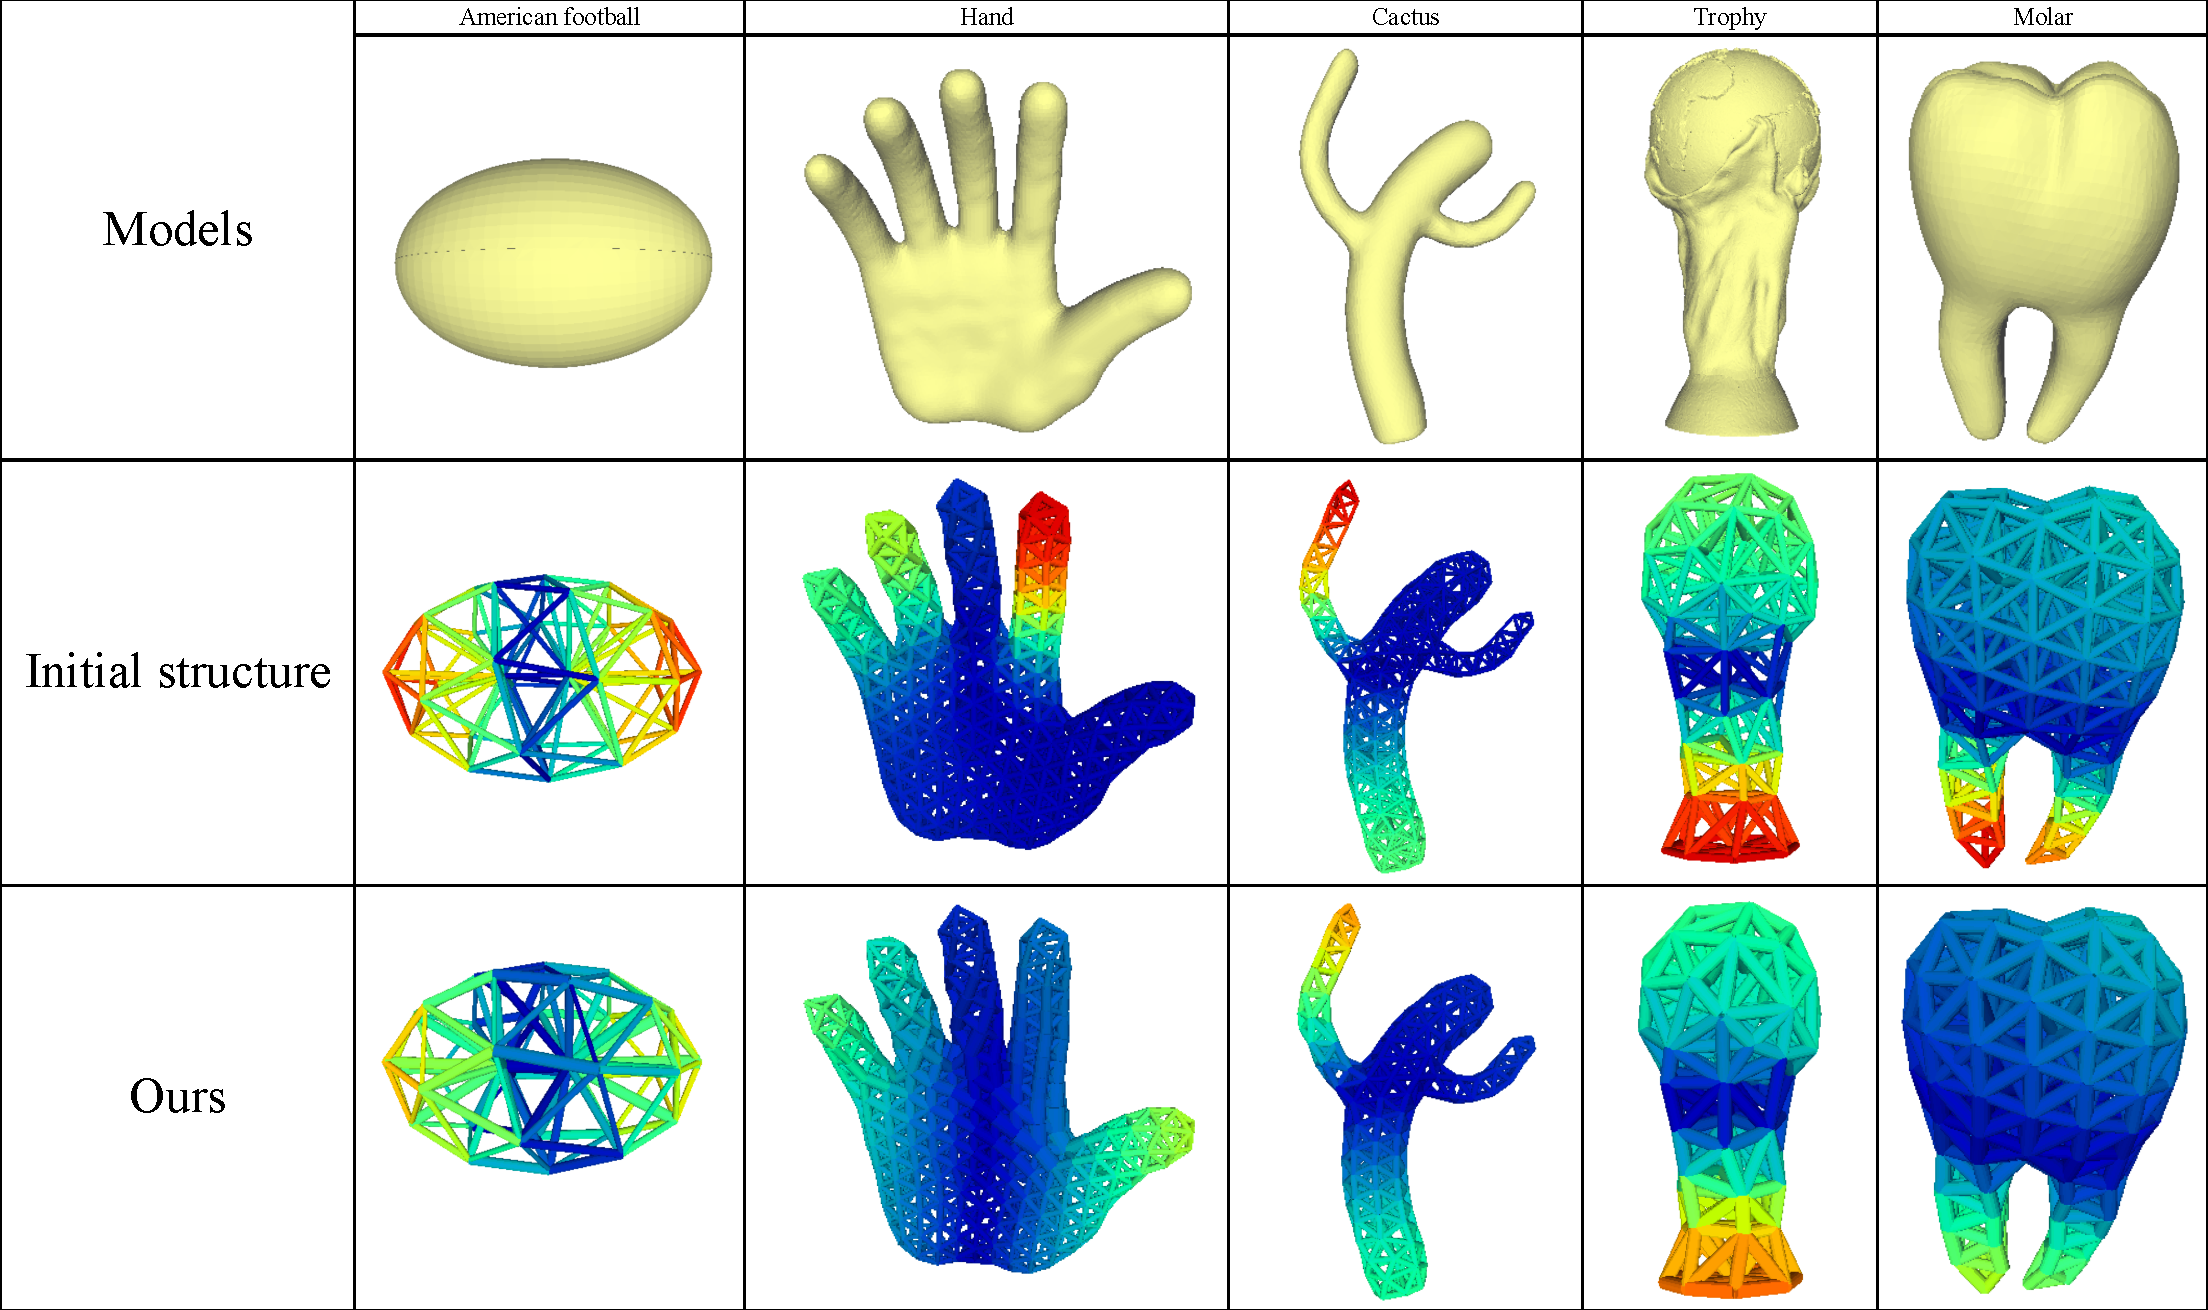
\includegraphics[width=.85\linewidth]{Figures/fig4/fig4.pdf}
    
\caption{\label{fig_frame_max}
  Maximum deformation distribution case for test frame structures.
            Top: Input model; Middle: distribution map of initial structure; Bottom: distribution map of our optimized structure.
            The magnitude of maximum deformation on our resulting structure is much smaller than that on the uniform initial frame structure. Note that, for example in the hand model, the worst case is changing during our optimization of the frame structures}
\end{figure*}

\begin{table}[htb]
\caption{\label{table_frame}Statistics of tests for frame structure. Mean values of 4000 records of deformation (in mm) for each model are listed. The maximum deformation value for each model is also listed. First two rows are the results of uniform frame and the last two rows are our results .}
\centering
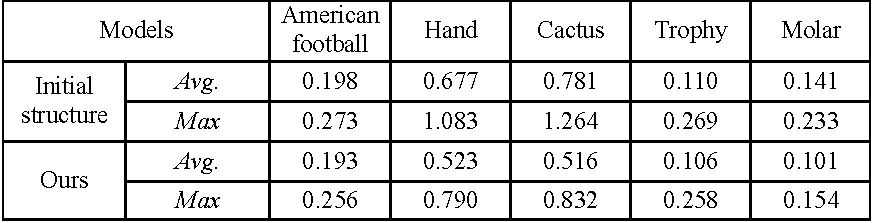
\includegraphics[width=0.5\linewidth]{Tables/table1}
\end{table}

\noindent\textbf{Physical experiment simulation} For examing the final object generated based on the optimized frame structure, FEM-based computation framework need to be adapted. For an elastic body $\Omega$, the stionary state of objects under forces can be described by the linear elasticity problem,
\begin{align}\label{eq:linear-elasticity}
     -\mbox{div}(\sigma(\epsilon(u))) & = f, \quad in\ \Omega \notag \\
                             u & = 0, \quad on\ \Gamma_D \\
          \sigma(\epsilon(u))\cdot n & = g, \quad on\ \Gamma_N. \notag
\end{align}
In this problem, $u$ is displacement, $\epsilon(u)=1/2(\nabla u+\nabla u^T)$ is the strain,
and $\sigma(\epsilon)=2\mu\epsilon+\gamma(\mathrm{tr}(\epsilon))I$ is the stress.
The quantities $\gamma$ and $\mu$ are the Lame moduli of the material. Such a problem can be solved by using FEMs. In our experiment, the FEM computation is executed by using DOLFIN~\cite{DOLFIN}.

We compare our results and uniform hollowing solution. In Fig.~\ref{fig_obj_hand}, we show the comparsion of the same cases as shown in Fig.~\ref{fig_frame_hand_case} for the hand model. General statistic data is shown in Table~\ref{table_obj}. We also compare our reuslt with \cite{Lu:2014}. We generate a global stiffness molar model which has the same volume with the molar example provided by this work as shown in Fig.~\ref{fig_cmp_btl}. 
%Two certain cases are shown in Fig.~\ref{fig_comp_btl}. 
The simluated results show that ours are more suitable under unknown load cases. 

\begin{figure}[h]
  \centering
  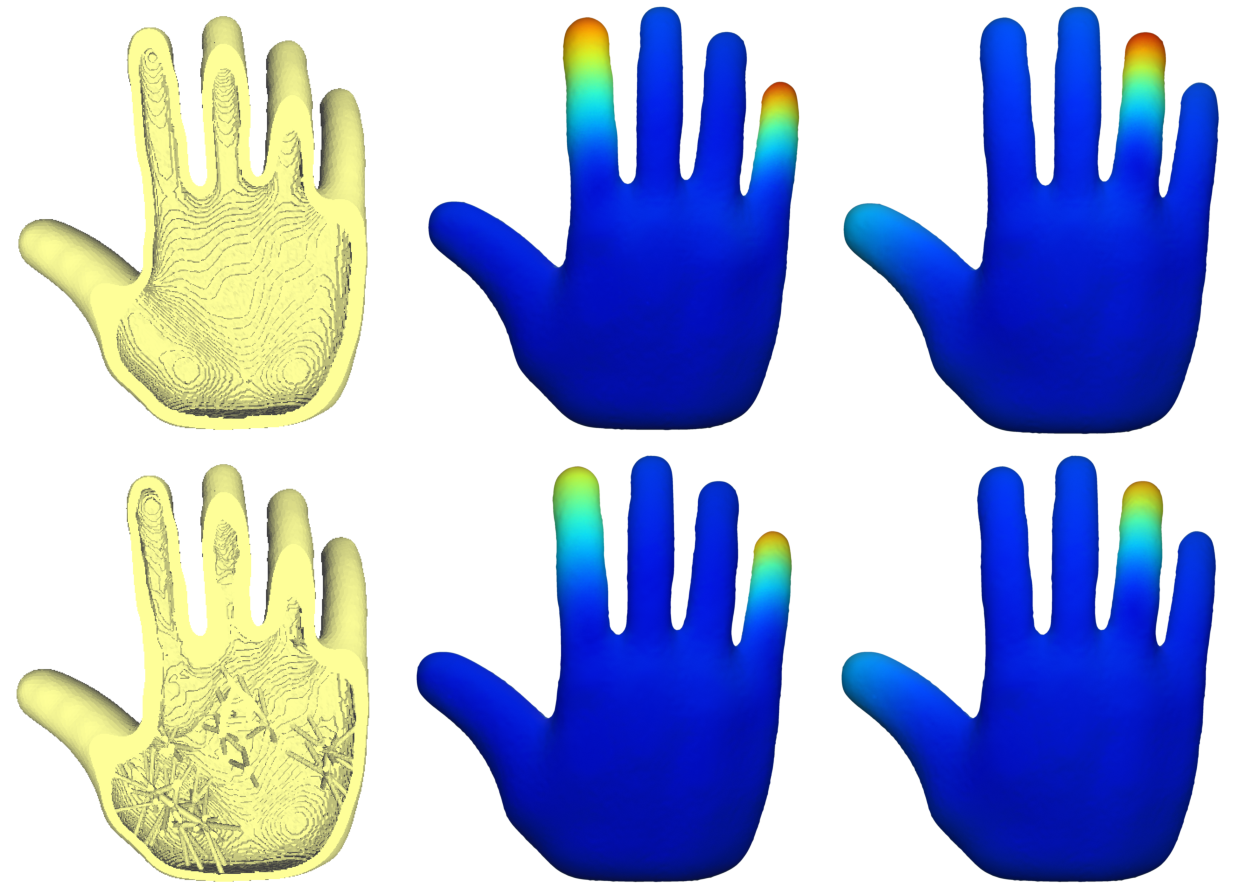
\includegraphics[width=0.5\linewidth]{Figures/hand/fig_obj_hand.pdf}
  \caption{\label{fig_obj_hand} Deformation distribution of the two load distribution cases (same as the cases shown in Fig.~\ref{fig_frame_hand_case}) on the uniform hollowing result (top) and our optimal result (bottom) of hand model. The first colume is the sectional view. The load is acted as pinching the forefinger and the little finger for the second colume and pinching the thumb and the third finger for the last colume. Two objects we tested have the same volume. It can be observe that the final object generated by our proposed postpocessing can sucessfully inherit the mechanical property and preforms better.}
\end{figure}

\begin{table}[htb]
\caption{\label{table_obj}Statistics of the simulation tests for object. Mean values of 4000 records of deformation (in mm) for each model are listed. The maximum deformation value for each model is also listed. First two rows are the results of uniform hollowing solution and the last two rows are our results .}
\centering
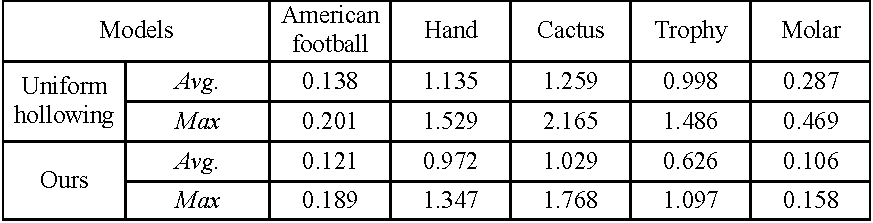
\includegraphics[width=0.5\linewidth]{Tables/table2}
\end{table}

\begin{figure}[h]
  \centering
  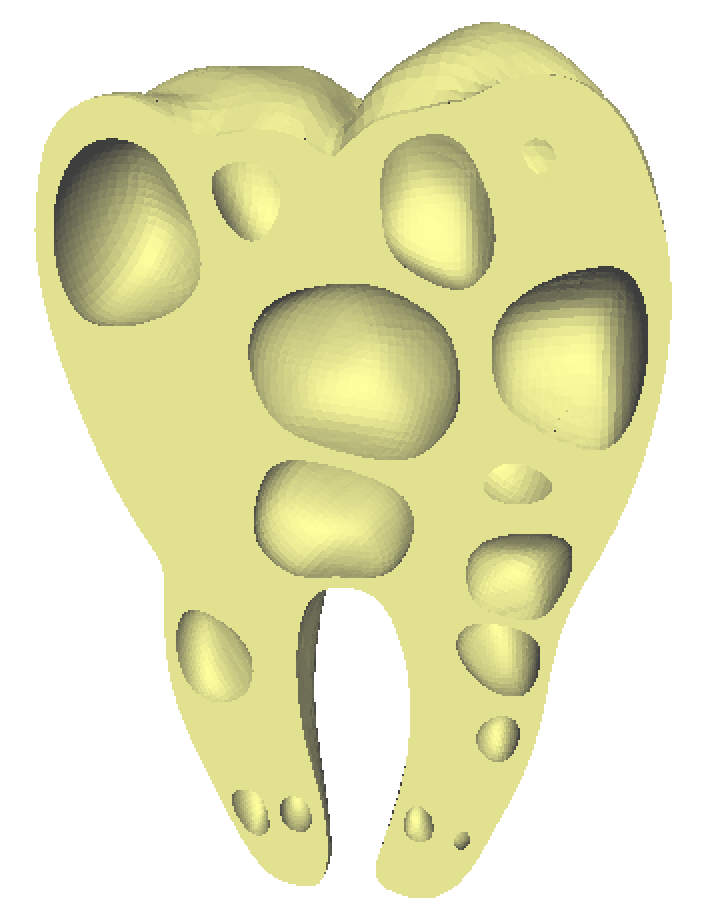
\includegraphics[width=0.2\linewidth]{Figures/molar_cmp/m2}
  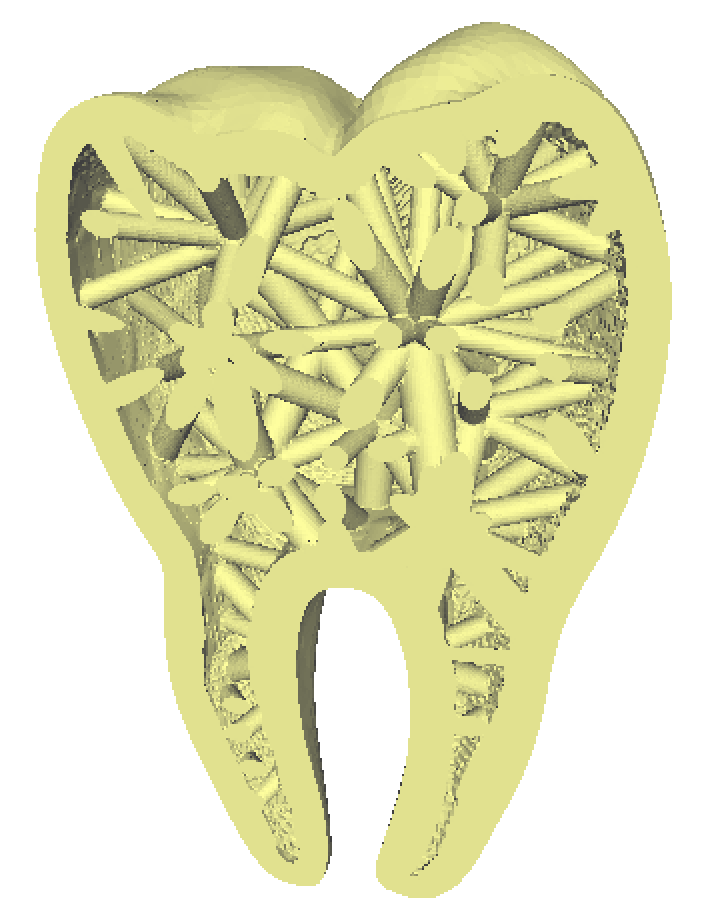
\includegraphics[width=0.2\linewidth]{Figures/molar_cmp/m1}

  \caption{\label{fig_cmp_btl} We compare our result with \cite{Lu:2014}. The left one is provided by \cite{Lu:2014} and the right one is ours. Two result objects have the same volume and the (Avg., Max) deformation is (0.125,0.197) and (0.106,0.158), respectively.}
\end{figure}

\begin{figure}[!h]
  \centering
  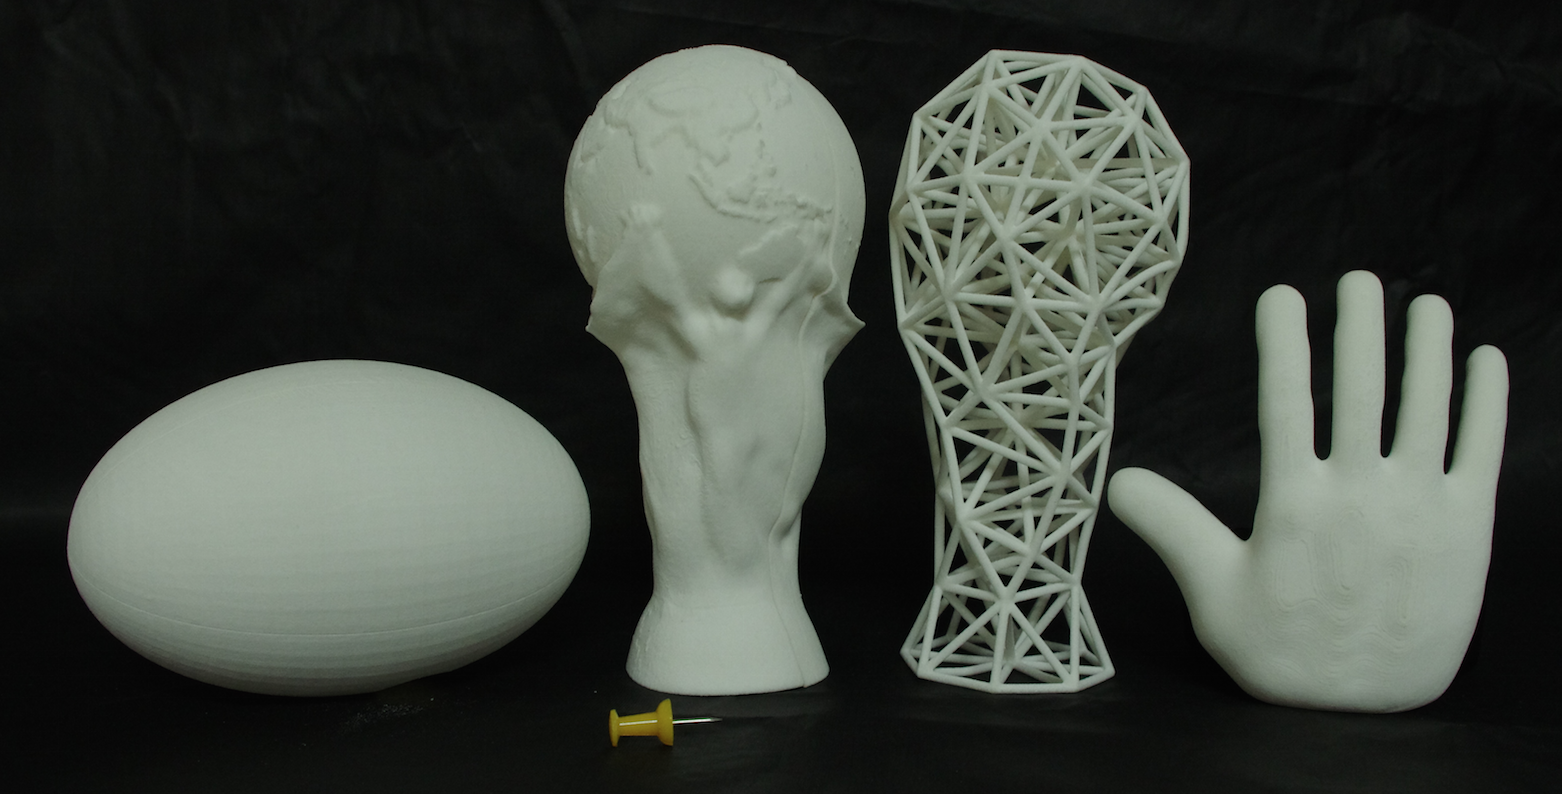
\includegraphics[width=0.5\linewidth]{Figures/results/1}
  \caption{\label{fig_all} We fabricate the final results for some models.}
\end{figure}

Our saddle point optimization problem can be solved very efficiently. All examples appear in this paper are optimized within 20mins.








\section{Conclusion}
\label{sec:conclusion}

In this work, we propose a novel approach for global stiffness struture optimization and present a saddle point algorithm to solve the optimization problem efficiently.
%
When given a certain amount of material for printing an object in 3D, our approach can generate a global stiffness structure with minimum deformation under all possible force distributions.
%
Our approach also provides a solution for formulating adaptive hollowing and interior supportive structures in a unifed form, while optimizing them simultaneously.
%
A number of experimental results have shown the validity and the rationality of our solution,
and have proved our proposed approach to be much more applicable than previous methods.
%


\noindent\textbf{Limitations and future work}
Our research opens several future studies in the direction of structural optimization.

In this paper, the optimization's objective is to minimize the possible deformation of objects.
However, the maximum stress distribution inside an object is of more interest in some applications, since it tells us where a crack is likely to happen. For such a need, we should introduce new objective functions. A simple idea is to consider the following optimization problem.
$$
\min_{(V,r)}\max_{f} \frac{\int_{\Omega} |\sigma|^2 dx}{\int_\Omega f^2dx}
$$
where $\sigma$ denotes the stress of the body under a force $f$.


%\xuefeng{My revision ends here.}


%From beam theory we know that lightweight frame structures under small load can be considered as linear elastic structure.
%Nonlinear elasticity has to be investigated for cases of frame under large deformation.
%In nonlinear elasticity, the displacements of nodes are not linearly related to the loads, so the linear stiffness equation is no longer valid.
%%
%
%%There are two dual problems in the structural optimization:
%%maximizing the strength of designed structure with given material volume constraint;
%%and minimizing the volume of material usage to meet a given strength/deformation constraint on the structure.
%
%
%In our current work, we consider the structural optimization problem of maximizing the global stiffness of designed structure with a given amount of material constraint.
%%
%Here the maximum global stiffness structure is defined as that provides minimal deformation under various force distribution.
%If we consider the maximum strength structure that produces minimal stress under various force distribution, the structural optimization problem appears to be solvable but would be challenging.
%%
%Second, .... some topic is an intriguing direction for future research.



%%%%%%%%%%%%%%%%%%%%%%%%%%%%%%%%%%%%%%%%%%%%%%%%%%%%%%%%%%%%%%%%%%%%

\bibliographystyle{abbrv}
\bibliography{structural}

\end{document}
